\documentclass{report}

%%%%%%%%%%%%%%%%%%%%%%%%%%%%%%%%%
% PACKAGE IMPORTS
%%%%%%%%%%%%%%%%%%%%%%%%%%%%%%%%%


\usepackage[tmargin=2cm,rmargin=1in,lmargin=1in,margin=0.85in,bmargin=2cm,footskip=.2in]{geometry}
\usepackage{amsmath,amsfonts,amsthm,amssymb,mathtools}
\usepackage[varbb]{newpxmath}
\usepackage{xfrac}
\usepackage[makeroom]{cancel}
\usepackage{mathtools}
\usepackage{bookmark}
\usepackage{enumitem}
\usepackage{hyperref,theoremref}
\hypersetup{
	pdftitle={Assignment},
	colorlinks=true, linkcolor=doc!90,
	bookmarksnumbered=true,
	bookmarksopen=true
}
\usepackage[most,many,breakable]{tcolorbox}
\usepackage{xcolor}
\usepackage{varwidth}
\usepackage{varwidth}
\usepackage{etoolbox}
%\usepackage{authblk}
\usepackage{nameref}
\usepackage{multicol,array}
\usepackage{tikz-cd}
\usepackage[ruled,vlined,linesnumbered]{algorithm2e}
\usepackage{comment} % enables the use of multi-line comments (\ifx \fi) 
\usepackage{import}
\usepackage{xifthen}
\usepackage{pdfpages}
\usepackage{transparent}

\newcommand\mycommfont[1]{\footnotesize\ttfamily\textcolor{blue}{#1}}
\SetCommentSty{mycommfont}
\newcommand{\incfig}[1]{%
    \def\svgwidth{\columnwidth}
    \import{./figures/}{#1.pdf_tex}
}

\usepackage{tikzsymbols}
\renewcommand\qedsymbol{$\Laughey$}


%\usepackage{import}
%\usepackage{xifthen}
%\usepackage{pdfpages}
%\usepackage{transparent}


%%%%%%%%%%%%%%%%%%%%%%%%%%%%%%
% SELF MADE COLORS
%%%%%%%%%%%%%%%%%%%%%%%%%%%%%%



\definecolor{myg}{RGB}{56, 140, 70}
\definecolor{myb}{RGB}{45, 111, 177}
\definecolor{myr}{RGB}{199, 68, 64}
\definecolor{mytheorembg}{HTML}{F2F2F9}
\definecolor{mytheoremfr}{HTML}{00007B}
\definecolor{mylenmabg}{HTML}{FFFAF8}
\definecolor{mylenmafr}{HTML}{983b0f}
\definecolor{mypropbg}{HTML}{f2fbfc}
\definecolor{mypropfr}{HTML}{191971}
\definecolor{myexamplebg}{HTML}{F2FBF8}
\definecolor{myexamplefr}{HTML}{88D6D1}
\definecolor{myexampleti}{HTML}{2A7F7F}
\definecolor{mydefinitbg}{HTML}{E5E5FF}
\definecolor{mydefinitfr}{HTML}{3F3FA3}
\definecolor{notesgreen}{RGB}{0,162,0}
\definecolor{myp}{RGB}{197, 92, 212}
\definecolor{mygr}{HTML}{2C3338}
\definecolor{myred}{RGB}{127,0,0}
\definecolor{myyellow}{RGB}{169,121,69}
\definecolor{myexercisebg}{HTML}{F2FBF8}
\definecolor{myexercisefg}{HTML}{88D6D1}


%%%%%%%%%%%%%%%%%%%%%%%%%%%%
% TCOLORBOX SETUPS
%%%%%%%%%%%%%%%%%%%%%%%%%%%%

\setlength{\parindent}{1cm}
%================================
% THEOREM BOX
%================================

\tcbuselibrary{theorems,skins,hooks}
\newtcbtheorem[number within=section]{Theorem}{Theorem}
{%
	enhanced,
	breakable,
	colback = mytheorembg,
	frame hidden,
	boxrule = 0sp,
	borderline west = {2pt}{0pt}{mytheoremfr},
	sharp corners,
	detach title,
	before upper = \tcbtitle\par\smallskip,
	coltitle = mytheoremfr,
	fonttitle = \bfseries\sffamily,
	description font = \mdseries,
	separator sign none,
	segmentation style={solid, mytheoremfr},
}
{th}

\tcbuselibrary{theorems,skins,hooks}
\newtcbtheorem[number within=chapter]{theorem}{Theorem}
{%
	enhanced,
	breakable,
	colback = mytheorembg,
	frame hidden,
	boxrule = 0sp,
	borderline west = {2pt}{0pt}{mytheoremfr},
	sharp corners,
	detach title,
	before upper = \tcbtitle\par\smallskip,
	coltitle = mytheoremfr,
	fonttitle = \bfseries\sffamily,
	description font = \mdseries,
	separator sign none,
	segmentation style={solid, mytheoremfr},
}
{th}


\tcbuselibrary{theorems,skins,hooks}
\newtcolorbox{Theoremcon}
{%
	enhanced
	,breakable
	,colback = mytheorembg
	,frame hidden
	,boxrule = 0sp
	,borderline west = {2pt}{0pt}{mytheoremfr}
	,sharp corners
	,description font = \mdseries
	,separator sign none
}

%================================
% Corollery
%================================
\tcbuselibrary{theorems,skins,hooks}
\newtcbtheorem[number within=section]{Corollary}{Corollary}
{%
	enhanced
	,breakable
	,colback = myp!10
	,frame hidden
	,boxrule = 0sp
	,borderline west = {2pt}{0pt}{myp!85!black}
	,sharp corners
	,detach title
	,before upper = \tcbtitle\par\smallskip
	,coltitle = myp!85!black
	,fonttitle = \bfseries\sffamily
	,description font = \mdseries
	,separator sign none
	,segmentation style={solid, myp!85!black}
}
{th}
\tcbuselibrary{theorems,skins,hooks}
\newtcbtheorem[number within=chapter]{corollary}{Corollary}
{%
	enhanced
	,breakable
	,colback = myp!10
	,frame hidden
	,boxrule = 0sp
	,borderline west = {2pt}{0pt}{myp!85!black}
	,sharp corners
	,detach title
	,before upper = \tcbtitle\par\smallskip
	,coltitle = myp!85!black
	,fonttitle = \bfseries\sffamily
	,description font = \mdseries
	,separator sign none
	,segmentation style={solid, myp!85!black}
}
{th}


%================================
% LENMA
%================================

\tcbuselibrary{theorems,skins,hooks}
\newtcbtheorem[number within=section]{Lenma}{Lenma}
{%
	enhanced,
	breakable,
	colback = mylenmabg,
	frame hidden,
	boxrule = 0sp,
	borderline west = {2pt}{0pt}{mylenmafr},
	sharp corners,
	detach title,
	before upper = \tcbtitle\par\smallskip,
	coltitle = mylenmafr,
	fonttitle = \bfseries\sffamily,
	description font = \mdseries,
	separator sign none,
	segmentation style={solid, mylenmafr},
}
{th}

\tcbuselibrary{theorems,skins,hooks}
\newtcbtheorem[number within=chapter]{lenma}{Lenma}
{%
	enhanced,
	breakable,
	colback = mylenmabg,
	frame hidden,
	boxrule = 0sp,
	borderline west = {2pt}{0pt}{mylenmafr},
	sharp corners,
	detach title,
	before upper = \tcbtitle\par\smallskip,
	coltitle = mylenmafr,
	fonttitle = \bfseries\sffamily,
	description font = \mdseries,
	separator sign none,
	segmentation style={solid, mylenmafr},
}
{th}


%================================
% PROPOSITION
%================================

\tcbuselibrary{theorems,skins,hooks}
\newtcbtheorem[number within=section]{Prop}{Proposition}
{%
	enhanced,
	breakable,
	colback = mypropbg,
	frame hidden,
	boxrule = 0sp,
	borderline west = {2pt}{0pt}{mypropfr},
	sharp corners,
	detach title,
	before upper = \tcbtitle\par\smallskip,
	coltitle = mypropfr,
	fonttitle = \bfseries\sffamily,
	description font = \mdseries,
	separator sign none,
	segmentation style={solid, mypropfr},
}
{th}

\tcbuselibrary{theorems,skins,hooks}
\newtcbtheorem[number within=chapter]{prop}{Proposition}
{%
	enhanced,
	breakable,
	colback = mypropbg,
	frame hidden,
	boxrule = 0sp,
	borderline west = {2pt}{0pt}{mypropfr},
	sharp corners,
	detach title,
	before upper = \tcbtitle\par\smallskip,
	coltitle = mypropfr,
	fonttitle = \bfseries\sffamily,
	description font = \mdseries,
	separator sign none,
	segmentation style={solid, mypropfr},
}
{th}


%================================
% CLAIM
%================================

\tcbuselibrary{theorems,skins,hooks}
\newtcbtheorem[number within=section]{claim}{Claim}
{%
	enhanced
	,breakable
	,colback = myg!10
	,frame hidden
	,boxrule = 0sp
	,borderline west = {2pt}{0pt}{myg}
	,sharp corners
	,detach title
	,before upper = \tcbtitle\par\smallskip
	,coltitle = myg!85!black
	,fonttitle = \bfseries\sffamily
	,description font = \mdseries
	,separator sign none
	,segmentation style={solid, myg!85!black}
}
{th}



%================================
% Exercise
%================================

\tcbuselibrary{theorems,skins,hooks}
\newtcbtheorem[number within=section]{Exercise}{Exercise}
{%
	enhanced,
	breakable,
	colback = myexercisebg,
	frame hidden,
	boxrule = 0sp,
	borderline west = {2pt}{0pt}{myexercisefg},
	sharp corners,
	detach title,
	before upper = \tcbtitle\par\smallskip,
	coltitle = myexercisefg,
	fonttitle = \bfseries\sffamily,
	description font = \mdseries,
	separator sign none,
	segmentation style={solid, myexercisefg},
}
{th}

\tcbuselibrary{theorems,skins,hooks}
\newtcbtheorem[number within=chapter]{exercise}{Exercise}
{%
	enhanced,
	breakable,
	colback = myexercisebg,
	frame hidden,
	boxrule = 0sp,
	borderline west = {2pt}{0pt}{myexercisefg},
	sharp corners,
	detach title,
	before upper = \tcbtitle\par\smallskip,
	coltitle = myexercisefg,
	fonttitle = \bfseries\sffamily,
	description font = \mdseries,
	separator sign none,
	segmentation style={solid, myexercisefg},
}
{th}

%================================
% EXAMPLE BOX
%================================

\newtcbtheorem[number within=section]{Example}{Example}
{%
	colback = myexamplebg
	,breakable
	,colframe = myexamplefr
	,coltitle = myexampleti
	,boxrule = 1pt
	,sharp corners
	,detach title
	,before upper=\tcbtitle\par\smallskip
	,fonttitle = \bfseries
	,description font = \mdseries
	,separator sign none
	,description delimiters parenthesis
}
{ex}

\newtcbtheorem[number within=chapter]{example}{Example}
{%
	colback = myexamplebg
	,breakable
	,colframe = myexamplefr
	,coltitle = myexampleti
	,boxrule = 1pt
	,sharp corners
	,detach title
	,before upper=\tcbtitle\par\smallskip
	,fonttitle = \bfseries
	,description font = \mdseries
	,separator sign none
	,description delimiters parenthesis
}
{ex}

%================================
% DEFINITION BOX
%================================

\newtcbtheorem[number within=section]{Definition}{Definition}{enhanced,
	before skip=2mm,after skip=2mm, colback=red!5,colframe=red!80!black,boxrule=0.5mm,
	attach boxed title to top left={xshift=1cm,yshift*=1mm-\tcboxedtitleheight}, varwidth boxed title*=-3cm,
	boxed title style={frame code={
					\path[fill=tcbcolback]
					([yshift=-1mm,xshift=-1mm]frame.north west)
					arc[start angle=0,end angle=180,radius=1mm]
					([yshift=-1mm,xshift=1mm]frame.north east)
					arc[start angle=180,end angle=0,radius=1mm];
					\path[left color=tcbcolback!60!black,right color=tcbcolback!60!black,
						middle color=tcbcolback!80!black]
					([xshift=-2mm]frame.north west) -- ([xshift=2mm]frame.north east)
					[rounded corners=1mm]-- ([xshift=1mm,yshift=-1mm]frame.north east)
					-- (frame.south east) -- (frame.south west)
					-- ([xshift=-1mm,yshift=-1mm]frame.north west)
					[sharp corners]-- cycle;
				},interior engine=empty,
		},
	fonttitle=\bfseries,
	title={#2},#1}{def}
\newtcbtheorem[number within=chapter]{definition}{Definition}{enhanced,
	before skip=2mm,after skip=2mm, colback=red!5,colframe=red!80!black,boxrule=0.5mm,
	attach boxed title to top left={xshift=1cm,yshift*=1mm-\tcboxedtitleheight}, varwidth boxed title*=-3cm,
	boxed title style={frame code={
					\path[fill=tcbcolback]
					([yshift=-1mm,xshift=-1mm]frame.north west)
					arc[start angle=0,end angle=180,radius=1mm]
					([yshift=-1mm,xshift=1mm]frame.north east)
					arc[start angle=180,end angle=0,radius=1mm];
					\path[left color=tcbcolback!60!black,right color=tcbcolback!60!black,
						middle color=tcbcolback!80!black]
					([xshift=-2mm]frame.north west) -- ([xshift=2mm]frame.north east)
					[rounded corners=1mm]-- ([xshift=1mm,yshift=-1mm]frame.north east)
					-- (frame.south east) -- (frame.south west)
					-- ([xshift=-1mm,yshift=-1mm]frame.north west)
					[sharp corners]-- cycle;
				},interior engine=empty,
		},
	fonttitle=\bfseries,
	title={#2},#1}{def}



%================================
% Solution BOX
%================================

\makeatletter
\newtcbtheorem{question}{Question}{enhanced,
	breakable,
	colback=white,
	colframe=myb!80!black,
	attach boxed title to top left={yshift*=-\tcboxedtitleheight},
	fonttitle=\bfseries,
	title={#2},
	boxed title size=title,
	boxed title style={%
			sharp corners,
			rounded corners=northwest,
			colback=tcbcolframe,
			boxrule=0pt,
		},
	underlay boxed title={%
			\path[fill=tcbcolframe] (title.south west)--(title.south east)
			to[out=0, in=180] ([xshift=5mm]title.east)--
			(title.center-|frame.east)
			[rounded corners=\kvtcb@arc] |-
			(frame.north) -| cycle;
		},
	#1
}{def}
\makeatother

%================================
% SOLUTION BOX
%================================

\makeatletter
\newtcolorbox{solution}{enhanced,
	breakable,
	colback=white,
	colframe=myg!80!black,
	attach boxed title to top left={yshift*=-\tcboxedtitleheight},
	title=Solution,
	boxed title size=title,
	boxed title style={%
			sharp corners,
			rounded corners=northwest,
			colback=tcbcolframe,
			boxrule=0pt,
		},
	underlay boxed title={%
			\path[fill=tcbcolframe] (title.south west)--(title.south east)
			to[out=0, in=180] ([xshift=5mm]title.east)--
			(title.center-|frame.east)
			[rounded corners=\kvtcb@arc] |-
			(frame.north) -| cycle;
		},
}
\makeatother

%================================
% Question BOX
%================================

\makeatletter
\newtcbtheorem{qstion}{Question}{enhanced,
	breakable,
	colback=white,
	colframe=mygr,
	attach boxed title to top left={yshift*=-\tcboxedtitleheight},
	fonttitle=\bfseries,
	title={#2},
	boxed title size=title,
	boxed title style={%
			sharp corners,
			rounded corners=northwest,
			colback=tcbcolframe,
			boxrule=0pt,
		},
	underlay boxed title={%
			\path[fill=tcbcolframe] (title.south west)--(title.south east)
			to[out=0, in=180] ([xshift=5mm]title.east)--
			(title.center-|frame.east)
			[rounded corners=\kvtcb@arc] |-
			(frame.north) -| cycle;
		},
	#1
}{def}
\makeatother

\newtcbtheorem[number within=chapter]{wconc}{Wrong Concept}{
	breakable,
	enhanced,
	colback=white,
	colframe=myr,
	arc=0pt,
	outer arc=0pt,
	fonttitle=\bfseries\sffamily\large,
	colbacktitle=myr,
	attach boxed title to top left={},
	boxed title style={
			enhanced,
			skin=enhancedfirst jigsaw,
			arc=3pt,
			bottom=0pt,
			interior style={fill=myr}
		},
	#1
}{def}



%================================
% NOTE BOX
%================================

\usetikzlibrary{arrows,calc,shadows.blur}
\tcbuselibrary{skins}
\newtcolorbox{note}[1][]{%
	enhanced jigsaw,
	colback=gray!20!white,%
	colframe=gray!80!black,
	size=small,
	boxrule=1pt,
	title=\textbf{Note:-},
	halign title=flush center,
	coltitle=black,
	breakable,
	drop shadow=black!50!white,
	attach boxed title to top left={xshift=1cm,yshift=-\tcboxedtitleheight/2,yshifttext=-\tcboxedtitleheight/2},
	minipage boxed title=1.5cm,
	boxed title style={%
			colback=white,
			size=fbox,
			boxrule=1pt,
			boxsep=2pt,
			underlay={%
					\coordinate (dotA) at ($(interior.west) + (-0.5pt,0)$);
					\coordinate (dotB) at ($(interior.east) + (0.5pt,0)$);
					\begin{scope}
						\clip (interior.north west) rectangle ([xshift=3ex]interior.east);
						\filldraw [white, blur shadow={shadow opacity=60, shadow yshift=-.75ex}, rounded corners=2pt] (interior.north west) rectangle (interior.south east);
					\end{scope}
					\begin{scope}[gray!80!black]
						\fill (dotA) circle (2pt);
						\fill (dotB) circle (2pt);
					\end{scope}
				},
		},
	#1,
}

%%%%%%%%%%%%%%%%%%%%%%%%%%%%%%
% SELF MADE COMMANDS
%%%%%%%%%%%%%%%%%%%%%%%%%%%%%%


\newcommand{\thm}[2]{\begin{Theorem}{#1}{}#2\end{Theorem}}
\newcommand{\cor}[2]{\begin{Corollary}{#1}{}#2\end{Corollary}}
\newcommand{\mlenma}[2]{\begin{Lenma}{#1}{}#2\end{Lenma}}
\newcommand{\mprop}[2]{\begin{Prop}{#1}{}#2\end{Prop}}
\newcommand{\clm}[3]{\begin{claim}{#1}{#2}#3\end{claim}}
\newcommand{\wc}[2]{\begin{wconc}{#1}{}\setlength{\parindent}{1cm}#2\end{wconc}}
\newcommand{\thmcon}[1]{\begin{Theoremcon}{#1}\end{Theoremcon}}
\newcommand{\ex}[2]{\begin{Example}{#1}{}#2\end{Example}}
\newcommand{\dfn}[2]{\begin{Definition}[colbacktitle=red!75!black]{#1}{}#2\end{Definition}}
\newcommand{\dfnc}[2]{\begin{definition}[colbacktitle=red!75!black]{#1}{}#2\end{definition}}
\newcommand{\qs}[2]{\begin{question}{#1}{}#2\end{question}}
\newcommand{\pf}[2]{\begin{myproof}[#1]#2\end{myproof}}
\newcommand{\nt}[1]{\begin{note}#1\end{note}}

\newcommand*\circled[1]{\tikz[baseline=(char.base)]{
		\node[shape=circle,draw,inner sep=1pt] (char) {#1};}}
\newcommand\getcurrentref[1]{%
	\ifnumequal{\value{#1}}{0}
	{??}
	{\the\value{#1}}%
}
\newcommand{\getCurrentSectionNumber}{\getcurrentref{section}}
\newenvironment{myproof}[1][\proofname]{%
	\proof[\bfseries #1: ]%
}{\endproof}

\newcommand{\mclm}[2]{\begin{myclaim}[#1]#2\end{myclaim}}
\newenvironment{myclaim}[1][\claimname]{\proof[\bfseries #1: ]}{}

\newcounter{mylabelcounter}

\makeatletter
\newcommand{\setword}[2]{%
	\phantomsection
	#1\def\@currentlabel{\unexpanded{#1}}\label{#2}%
}
\makeatother




\tikzset{
	symbol/.style={
			draw=none,
			every to/.append style={
					edge node={node [sloped, allow upside down, auto=false]{$#1$}}}
		}
}


% deliminators
\DeclarePairedDelimiter{\abs}{\lvert}{\rvert}
\DeclarePairedDelimiter{\norm}{\lVert}{\rVert}

\DeclarePairedDelimiter{\ceil}{\lceil}{\rceil}
\DeclarePairedDelimiter{\floor}{\lfloor}{\rfloor}
\DeclarePairedDelimiter{\round}{\lfloor}{\rceil}

\newsavebox\diffdbox
\newcommand{\slantedromand}{{\mathpalette\makesl{d}}}
\newcommand{\makesl}[2]{%
\begingroup
\sbox{\diffdbox}{$\mathsurround=0pt#1\mathrm{#2}$}%
\pdfsave
\pdfsetmatrix{1 0 0.2 1}%
\rlap{\usebox{\diffdbox}}%
\pdfrestore
\hskip\wd\diffdbox
\endgroup
}
\newcommand{\dd}[1][]{\ensuremath{\mathop{}\!\ifstrempty{#1}{%
\slantedromand\@ifnextchar^{\hspace{0.2ex}}{\hspace{0.1ex}}}%
{\slantedromand\hspace{0.2ex}^{#1}}}}
\ProvideDocumentCommand\dv{o m g}{%
  \ensuremath{%
    \IfValueTF{#3}{%
      \IfNoValueTF{#1}{%
        \frac{\dd #2}{\dd #3}%
      }{%
        \frac{\dd^{#1} #2}{\dd #3^{#1}}%
      }%
    }{%
      \IfNoValueTF{#1}{%
        \frac{\dd}{\dd #2}%
      }{%
        \frac{\dd^{#1}}{\dd #2^{#1}}%
      }%
    }%
  }%
}
\providecommand*{\pdv}[3][]{\frac{\partial^{#1}#2}{\partial#3^{#1}}}
%  - others
\DeclareMathOperator{\Lap}{\mathcal{L}}
\DeclareMathOperator{\Var}{Var} % varience
\DeclareMathOperator{\Cov}{Cov} % covarience
\DeclareMathOperator{\E}{E} % expected

% Since the amsthm package isn't loaded

% I prefer the slanted \leq
\let\oldleq\leq % save them in case they're every wanted
\let\oldgeq\geq
\renewcommand{\leq}{\leqslant}
\renewcommand{\geq}{\geqslant}

% % redefine matrix env to allow for alignment, use r as default
% \renewcommand*\env@matrix[1][r]{\hskip -\arraycolsep
%     \let\@ifnextchar\new@ifnextchar
%     \array{*\c@MaxMatrixCols #1}}


%\usepackage{framed}
%\usepackage{titletoc}
%\usepackage{etoolbox}
%\usepackage{lmodern}


%\patchcmd{\tableofcontents}{\contentsname}{\sffamily\contentsname}{}{}

%\renewenvironment{leftbar}
%{\def\FrameCommand{\hspace{6em}%
%		{\color{myyellow}\vrule width 2pt depth 6pt}\hspace{1em}}%
%	\MakeFramed{\parshape 1 0cm \dimexpr\textwidth-6em\relax\FrameRestore}\vskip2pt%
%}
%{\endMakeFramed}

%\titlecontents{chapter}
%[0em]{\vspace*{2\baselineskip}}
%{\parbox{4.5em}{%
%		\hfill\Huge\sffamily\bfseries\color{myred}\thecontentspage}%
%	\vspace*{-2.3\baselineskip}\leftbar\textsc{\small\chaptername~\thecontentslabel}\\\sffamily}
%{}{\endleftbar}
%\titlecontents{section}
%[8.4em]
%{\sffamily\contentslabel{3em}}{}{}
%{\hspace{0.5em}\nobreak\itshape\color{myred}\contentspage}
%\titlecontents{subsection}
%[8.4em]
%{\sffamily\contentslabel{3em}}{}{}  
%{\hspace{0.5em}\nobreak\itshape\color{myred}\contentspage}



%%%%%%%%%%%%%%%%%%%%%%%%%%%%%%%%%%%%%%%%%%%
% TABLE OF CONTENTS
%%%%%%%%%%%%%%%%%%%%%%%%%%%%%%%%%%%%%%%%%%%

\usepackage{tikz}
\definecolor{doc}{RGB}{0,60,110}
\usepackage{titletoc}
\contentsmargin{0cm}
\titlecontents{chapter}[3.7pc]
{\addvspace{30pt}%
	\begin{tikzpicture}[remember picture, overlay]%
		\draw[fill=doc!60,draw=doc!60] (-7,-.1) rectangle (-0.9,.5);%
		\pgftext[left,x=-3.5cm,y=0.2cm]{\color{white}\Large\sc\bfseries Chapter\ \thecontentslabel};%
	\end{tikzpicture}\color{doc!60}\large\sc\bfseries}%
{}
{}
{\;\titlerule\;\large\sc\bfseries Page \thecontentspage
	\begin{tikzpicture}[remember picture, overlay]
		\draw[fill=doc!60,draw=doc!60] (2pt,0) rectangle (4,0.1pt);
	\end{tikzpicture}}%
\titlecontents{section}[3.7pc]
{\addvspace{2pt}}
{\contentslabel[\thecontentslabel]{2pc}}
{}
{\hfill\small \thecontentspage}
[]
\titlecontents*{subsection}[3.7pc]
{\addvspace{-1pt}\small}
{}
{}
{\ --- \small\thecontentspage}
[ \textbullet\ ][]

\makeatletter
\renewcommand{\tableofcontents}{%
	\chapter*{%
	  \vspace*{-20\p@}%
	  \begin{tikzpicture}[remember picture, overlay]%
		  \pgftext[right,x=15cm,y=0.2cm]{\color{doc!60}\Huge\sc\bfseries \contentsname};%
		  \draw[fill=doc!60,draw=doc!60] (13,-.75) rectangle (20,1);%
		  \clip (13,-.75) rectangle (20,1);
		  \pgftext[right,x=15cm,y=0.2cm]{\color{white}\Huge\sc\bfseries \contentsname};%
	  \end{tikzpicture}}%
	\@starttoc{toc}}
\makeatother


%From M275 "Topology" at SJSU
\newcommand{\id}{\mathrm{id}}
\newcommand{\taking}[1]{\xrightarrow{#1}}
\newcommand{\inv}{^{-1}}

%From M170 "Introduction to Graph Theory" at SJSU
\DeclareMathOperator{\diam}{diam}
\DeclareMathOperator{\ord}{ord}
\newcommand{\defeq}{\overset{\mathrm{def}}{=}}

%From the USAMO .tex files
\newcommand{\ts}{\textsuperscript}
\newcommand{\dg}{^\circ}
\newcommand{\ii}{\item}

% % From Math 55 and Math 145 at Harvard
% \newenvironment{subproof}[1][Proof]{%
% \begin{proof}[#1] \renewcommand{\qedsymbol}{$\blacksquare$}}%
% {\end{proof}}

\newcommand{\liff}{\leftrightarrow}
\newcommand{\lthen}{\rightarrow}
\newcommand{\opname}{\operatorname}
\newcommand{\surjto}{\twoheadrightarrow}
\newcommand{\injto}{\hookrightarrow}
\newcommand{\On}{\mathrm{On}} % ordinals
\DeclareMathOperator{\img}{im} % Image
\DeclareMathOperator{\Img}{Im} % Image
\DeclareMathOperator{\coker}{coker} % Cokernel
\DeclareMathOperator{\Coker}{Coker} % Cokernel
\DeclareMathOperator{\Ker}{Ker} % Kernel
\DeclareMathOperator{\rank}{rank}
\DeclareMathOperator{\Spec}{Spec} % spectrum
\DeclareMathOperator{\Tr}{Tr} % trace
\DeclareMathOperator{\pr}{pr} % projection
\DeclareMathOperator{\ext}{ext} % extension
\DeclareMathOperator{\pred}{pred} % predecessor
\DeclareMathOperator{\dom}{dom} % domain
\DeclareMathOperator{\ran}{ran} % range
\DeclareMathOperator{\Hom}{Hom} % homomorphism
\DeclareMathOperator{\Mor}{Mor} % morphisms
\DeclareMathOperator{\End}{End} % endomorphism

\newcommand{\eps}{\epsilon}
\newcommand{\veps}{\varepsilon}
\newcommand{\ol}{\overline}
\newcommand{\ul}{\underline}
\newcommand{\wt}{\widetilde}
\newcommand{\wh}{\widehat}
\newcommand{\vocab}[1]{\textbf{\color{blue} #1}}
\providecommand{\half}{\frac{1}{2}}
\newcommand{\dang}{\measuredangle} %% Directed angle
\newcommand{\ray}[1]{\overrightarrow{#1}}
\newcommand{\seg}[1]{\overline{#1}}
\newcommand{\arc}[1]{\wideparen{#1}}
\DeclareMathOperator{\cis}{cis}
\DeclareMathOperator*{\lcm}{lcm}
\DeclareMathOperator*{\argmin}{arg min}
\DeclareMathOperator*{\argmax}{arg max}
\newcommand{\cycsum}{\sum_{\mathrm{cyc}}}
\newcommand{\symsum}{\sum_{\mathrm{sym}}}
\newcommand{\cycprod}{\prod_{\mathrm{cyc}}}
\newcommand{\symprod}{\prod_{\mathrm{sym}}}
\newcommand{\Qed}{\begin{flushright}\qed\end{flushright}}
\newcommand{\parinn}{\setlength{\parindent}{1cm}}
\newcommand{\parinf}{\setlength{\parindent}{0cm}}
% \newcommand{\norm}{\|\cdot\|}
\newcommand{\inorm}{\norm_{\infty}}
\newcommand{\opensets}{\{V_{\alpha}\}_{\alpha\in I}}
\newcommand{\oset}{V_{\alpha}}
\newcommand{\opset}[1]{V_{\alpha_{#1}}}
\newcommand{\lub}{\text{lub}}
\newcommand{\del}[2]{\frac{\partial #1}{\partial #2}}
\newcommand{\Del}[3]{\frac{\partial^{#1} #2}{\partial^{#1} #3}}
\newcommand{\deld}[2]{\dfrac{\partial #1}{\partial #2}}
\newcommand{\Deld}[3]{\dfrac{\partial^{#1} #2}{\partial^{#1} #3}}
\newcommand{\lm}{\lambda}
\newcommand{\uin}{\mathbin{\rotatebox[origin=c]{90}{$\in$}}}
\newcommand{\usubset}{\mathbin{\rotatebox[origin=c]{90}{$\subset$}}}
\newcommand{\lt}{\left}
\newcommand{\rt}{\right}
\newcommand{\bs}[1]{\boldsymbol{#1}}
\newcommand{\exs}{\exists}
\newcommand{\st}{\strut}
\newcommand{\dps}[1]{\displaystyle{#1}}

\newcommand{\sol}{\setlength{\parindent}{0cm}\textbf{\textit{Solution:}}\setlength{\parindent}{1cm} }
\newcommand{\solve}[1]{\setlength{\parindent}{0cm}\textbf{\textit{Solution: }}\setlength{\parindent}{1cm}#1 \Qed}

% Things Lie
\newcommand{\kb}{\mathfrak b}
\newcommand{\kg}{\mathfrak g}
\newcommand{\kh}{\mathfrak h}
\newcommand{\kn}{\mathfrak n}
\newcommand{\ku}{\mathfrak u}
\newcommand{\kz}{\mathfrak z}
\DeclareMathOperator{\Ext}{Ext} % Ext functor
\DeclareMathOperator{\Tor}{Tor} % Tor functor
\newcommand{\gl}{\opname{\mathfrak{gl}}} % frak gl group
\renewcommand{\sl}{\opname{\mathfrak{sl}}} % frak sl group chktex 6

% More script letters etc.
\newcommand{\SA}{\mathcal A}
\newcommand{\SB}{\mathcal B}
\newcommand{\SC}{\mathcal C}
\newcommand{\SF}{\mathcal F}
\newcommand{\SG}{\mathcal G}
\newcommand{\SH}{\mathcal H}
\newcommand{\OO}{\mathcal O}

\newcommand{\SCA}{\mathscr A}
\newcommand{\SCB}{\mathscr B}
\newcommand{\SCC}{\mathscr C}
\newcommand{\SCD}{\mathscr D}
\newcommand{\SCE}{\mathscr E}
\newcommand{\SCF}{\mathscr F}
\newcommand{\SCG}{\mathscr G}
\newcommand{\SCH}{\mathscr H}

% Mathfrak primes
\newcommand{\km}{\mathfrak m}
\newcommand{\kp}{\mathfrak p}
\newcommand{\kq}{\mathfrak q}

% number sets
\newcommand{\RR}[1][]{\ensuremath{\ifstrempty{#1}{\mathbb{R}}{\mathbb{R}^{#1}}}}
\newcommand{\NN}[1][]{\ensuremath{\ifstrempty{#1}{\mathbb{N}}{\mathbb{N}^{#1}}}}
\newcommand{\ZZ}[1][]{\ensuremath{\ifstrempty{#1}{\mathbb{Z}}{\mathbb{Z}^{#1}}}}
\newcommand{\QQ}[1][]{\ensuremath{\ifstrempty{#1}{\mathbb{Q}}{\mathbb{Q}^{#1}}}}
\newcommand{\CC}[1][]{\ensuremath{\ifstrempty{#1}{\mathbb{C}}{\mathbb{C}^{#1}}}}
\newcommand{\PP}[1][]{\ensuremath{\ifstrempty{#1}{\mathbb{P}}{\mathbb{P}^{#1}}}}
\newcommand{\HH}[1][]{\ensuremath{\ifstrempty{#1}{\mathbb{H}}{\mathbb{H}^{#1}}}}
\newcommand{\FF}[1][]{\ensuremath{\ifstrempty{#1}{\mathbb{F}}{\mathbb{F}^{#1}}}}
% expected value
\newcommand{\EE}{\ensuremath{\mathbb{E}}}
\newcommand{\charin}{\text{ char }}
\DeclareMathOperator{\sign}{sign}
\DeclareMathOperator{\Aut}{Aut}
\DeclareMathOperator{\Inn}{Inn}
\DeclareMathOperator{\Syl}{Syl}
\DeclareMathOperator{\Gal}{Gal}
\DeclareMathOperator{\GL}{GL} % General linear group
\DeclareMathOperator{\SL}{SL} % Special linear group

%---------------------------------------
% BlackBoard Math Fonts :-
%---------------------------------------

%Captital Letters
\newcommand{\bbA}{\mathbb{A}}	\newcommand{\bbB}{\mathbb{B}}
\newcommand{\bbC}{\mathbb{C}}	\newcommand{\bbD}{\mathbb{D}}
\newcommand{\bbE}{\mathbb{E}}	\newcommand{\bbF}{\mathbb{F}}
\newcommand{\bbG}{\mathbb{G}}	\newcommand{\bbH}{\mathbb{H}}
\newcommand{\bbI}{\mathbb{I}}	\newcommand{\bbJ}{\mathbb{J}}
\newcommand{\bbK}{\mathbb{K}}	\newcommand{\bbL}{\mathbb{L}}
\newcommand{\bbM}{\mathbb{M}}	\newcommand{\bbN}{\mathbb{N}}
\newcommand{\bbO}{\mathbb{O}}	\newcommand{\bbP}{\mathbb{P}}
\newcommand{\bbQ}{\mathbb{Q}}	\newcommand{\bbR}{\mathbb{R}}
\newcommand{\bbS}{\mathbb{S}}	\newcommand{\bbT}{\mathbb{T}}
\newcommand{\bbU}{\mathbb{U}}	\newcommand{\bbV}{\mathbb{V}}
\newcommand{\bbW}{\mathbb{W}}	\newcommand{\bbX}{\mathbb{X}}
\newcommand{\bbY}{\mathbb{Y}}	\newcommand{\bbZ}{\mathbb{Z}}

%---------------------------------------
% MathCal Fonts :-
%---------------------------------------

%Captital Letters
\newcommand{\mcA}{\mathcal{A}}	\newcommand{\mcB}{\mathcal{B}}
\newcommand{\mcC}{\mathcal{C}}	\newcommand{\mcD}{\mathcal{D}}
\newcommand{\mcE}{\mathcal{E}}	\newcommand{\mcF}{\mathcal{F}}
\newcommand{\mcG}{\mathcal{G}}	\newcommand{\mcH}{\mathcal{H}}
\newcommand{\mcI}{\mathcal{I}}	\newcommand{\mcJ}{\mathcal{J}}
\newcommand{\mcK}{\mathcal{K}}	\newcommand{\mcL}{\mathcal{L}}
\newcommand{\mcM}{\mathcal{M}}	\newcommand{\mcN}{\mathcal{N}}
\newcommand{\mcO}{\mathcal{O}}	\newcommand{\mcP}{\mathcal{P}}
\newcommand{\mcQ}{\mathcal{Q}}	\newcommand{\mcR}{\mathcal{R}}
\newcommand{\mcS}{\mathcal{S}}	\newcommand{\mcT}{\mathcal{T}}
\newcommand{\mcU}{\mathcal{U}}	\newcommand{\mcV}{\mathcal{V}}
\newcommand{\mcW}{\mathcal{W}}	\newcommand{\mcX}{\mathcal{X}}
\newcommand{\mcY}{\mathcal{Y}}	\newcommand{\mcZ}{\mathcal{Z}}


%---------------------------------------
% Bold Math Fonts :-
%---------------------------------------

%Captital Letters
\newcommand{\bmA}{\boldsymbol{A}}	\newcommand{\bmB}{\boldsymbol{B}}
\newcommand{\bmC}{\boldsymbol{C}}	\newcommand{\bmD}{\boldsymbol{D}}
\newcommand{\bmE}{\boldsymbol{E}}	\newcommand{\bmF}{\boldsymbol{F}}
\newcommand{\bmG}{\boldsymbol{G}}	\newcommand{\bmH}{\boldsymbol{H}}
\newcommand{\bmI}{\boldsymbol{I}}	\newcommand{\bmJ}{\boldsymbol{J}}
\newcommand{\bmK}{\boldsymbol{K}}	\newcommand{\bmL}{\boldsymbol{L}}
\newcommand{\bmM}{\boldsymbol{M}}	\newcommand{\bmN}{\boldsymbol{N}}
\newcommand{\bmO}{\boldsymbol{O}}	\newcommand{\bmP}{\boldsymbol{P}}
\newcommand{\bmQ}{\boldsymbol{Q}}	\newcommand{\bmR}{\boldsymbol{R}}
\newcommand{\bmS}{\boldsymbol{S}}	\newcommand{\bmT}{\boldsymbol{T}}
\newcommand{\bmU}{\boldsymbol{U}}	\newcommand{\bmV}{\boldsymbol{V}}
\newcommand{\bmW}{\boldsymbol{W}}	\newcommand{\bmX}{\boldsymbol{X}}
\newcommand{\bmY}{\boldsymbol{Y}}	\newcommand{\bmZ}{\boldsymbol{Z}}
%Small Letters
\newcommand{\bma}{\boldsymbol{a}}	\newcommand{\bmb}{\boldsymbol{b}}
\newcommand{\bmc}{\boldsymbol{c}}	\newcommand{\bmd}{\boldsymbol{d}}
\newcommand{\bme}{\boldsymbol{e}}	\newcommand{\bmf}{\boldsymbol{f}}
\newcommand{\bmg}{\boldsymbol{g}}	\newcommand{\bmh}{\boldsymbol{h}}
\newcommand{\bmi}{\boldsymbol{i}}	\newcommand{\bmj}{\boldsymbol{j}}
\newcommand{\bmk}{\boldsymbol{k}}	\newcommand{\bml}{\boldsymbol{l}}
\newcommand{\bmm}{\boldsymbol{m}}	\newcommand{\bmn}{\boldsymbol{n}}
\newcommand{\bmo}{\boldsymbol{o}}	\newcommand{\bmp}{\boldsymbol{p}}
\newcommand{\bmq}{\boldsymbol{q}}	\newcommand{\bmr}{\boldsymbol{r}}
\newcommand{\bms}{\boldsymbol{s}}	\newcommand{\bmt}{\boldsymbol{t}}
\newcommand{\bmu}{\boldsymbol{u}}	\newcommand{\bmv}{\boldsymbol{v}}
\newcommand{\bmw}{\boldsymbol{w}}	\newcommand{\bmx}{\boldsymbol{x}}
\newcommand{\bmy}{\boldsymbol{y}}	\newcommand{\bmz}{\boldsymbol{z}}

%---------------------------------------
% Scr Math Fonts :-
%---------------------------------------

\newcommand{\sA}{{\mathscr{A}}}   \newcommand{\sB}{{\mathscr{B}}}
\newcommand{\sC}{{\mathscr{C}}}   \newcommand{\sD}{{\mathscr{D}}}
\newcommand{\sE}{{\mathscr{E}}}   \newcommand{\sF}{{\mathscr{F}}}
\newcommand{\sG}{{\mathscr{G}}}   \newcommand{\sH}{{\mathscr{H}}}
\newcommand{\sI}{{\mathscr{I}}}   \newcommand{\sJ}{{\mathscr{J}}}
\newcommand{\sK}{{\mathscr{K}}}   \newcommand{\sL}{{\mathscr{L}}}
\newcommand{\sM}{{\mathscr{M}}}   \newcommand{\sN}{{\mathscr{N}}}
\newcommand{\sO}{{\mathscr{O}}}   \newcommand{\sP}{{\mathscr{P}}}
\newcommand{\sQ}{{\mathscr{Q}}}   \newcommand{\sR}{{\mathscr{R}}}
\newcommand{\sS}{{\mathscr{S}}}   \newcommand{\sT}{{\mathscr{T}}}
\newcommand{\sU}{{\mathscr{U}}}   \newcommand{\sV}{{\mathscr{V}}}
\newcommand{\sW}{{\mathscr{W}}}   \newcommand{\sX}{{\mathscr{X}}}
\newcommand{\sY}{{\mathscr{Y}}}   \newcommand{\sZ}{{\mathscr{Z}}}


%---------------------------------------
% Math Fraktur Font
%---------------------------------------

%Captital Letters
\newcommand{\mfA}{\mathfrak{A}}	\newcommand{\mfB}{\mathfrak{B}}
\newcommand{\mfC}{\mathfrak{C}}	\newcommand{\mfD}{\mathfrak{D}}
\newcommand{\mfE}{\mathfrak{E}}	\newcommand{\mfF}{\mathfrak{F}}
\newcommand{\mfG}{\mathfrak{G}}	\newcommand{\mfH}{\mathfrak{H}}
\newcommand{\mfI}{\mathfrak{I}}	\newcommand{\mfJ}{\mathfrak{J}}
\newcommand{\mfK}{\mathfrak{K}}	\newcommand{\mfL}{\mathfrak{L}}
\newcommand{\mfM}{\mathfrak{M}}	\newcommand{\mfN}{\mathfrak{N}}
\newcommand{\mfO}{\mathfrak{O}}	\newcommand{\mfP}{\mathfrak{P}}
\newcommand{\mfQ}{\mathfrak{Q}}	\newcommand{\mfR}{\mathfrak{R}}
\newcommand{\mfS}{\mathfrak{S}}	\newcommand{\mfT}{\mathfrak{T}}
\newcommand{\mfU}{\mathfrak{U}}	\newcommand{\mfV}{\mathfrak{V}}
\newcommand{\mfW}{\mathfrak{W}}	\newcommand{\mfX}{\mathfrak{X}}
\newcommand{\mfY}{\mathfrak{Y}}	\newcommand{\mfZ}{\mathfrak{Z}}
%Small Letters
\newcommand{\mfa}{\mathfrak{a}}	\newcommand{\mfb}{\mathfrak{b}}
\newcommand{\mfc}{\mathfrak{c}}	\newcommand{\mfd}{\mathfrak{d}}
\newcommand{\mfe}{\mathfrak{e}}	\newcommand{\mff}{\mathfrak{f}}
\newcommand{\mfg}{\mathfrak{g}}	\newcommand{\mfh}{\mathfrak{h}}
\newcommand{\mfi}{\mathfrak{i}}	\newcommand{\mfj}{\mathfrak{j}}
\newcommand{\mfk}{\mathfrak{k}}	\newcommand{\mfl}{\mathfrak{l}}
\newcommand{\mfm}{\mathfrak{m}}	\newcommand{\mfn}{\mathfrak{n}}
\newcommand{\mfo}{\mathfrak{o}}	\newcommand{\mfp}{\mathfrak{p}}
\newcommand{\mfq}{\mathfrak{q}}	\newcommand{\mfr}{\mathfrak{r}}
\newcommand{\mfs}{\mathfrak{s}}	\newcommand{\mft}{\mathfrak{t}}
\newcommand{\mfu}{\mathfrak{u}}	\newcommand{\mfv}{\mathfrak{v}}
\newcommand{\mfw}{\mathfrak{w}}	\newcommand{\mfx}{\mathfrak{x}}
\newcommand{\mfy}{\mathfrak{y}}	\newcommand{\mfz}{\mathfrak{z}}


\usepackage{tikz}
\usepackage{tikz-3dplot}
\usepackage{amsmath}
\usepackage{pgfplots}
\usepackage{smartdiagram}
\usesmartdiagramlibrary{additions}
\usepackage{xcolor}
\usepackage{forest}
\usepgfplotslibrary{colormaps}
\usepgfplotslibrary{groupplots}
\usepgfplotslibrary{polar}
\pgfplotsset{compat=newest}
\tikzset{>=latex}
\usepackage{siunitx}

\title{\Huge{MA193}\\Discrete Mathematics}
\author{\huge{Giacomo Cappelletto}}
\date{21/1/25}

\begin{document}


\maketitle
\newpage
\pdfbookmark[section]{\contentsname}{toc}
\tableofcontents
\pagebreak

\chapter{Fundamental Principles of Counting}

\section{Counting with Repetitions}

\nt{
	These notes cover the basic counting principles (often called the
	``Rule of Sum'' and the ``Rule of Product''), along with a brief
	discussion of permutations and combinations, including the formula
	for permutations of multiset objects (i.e., repeated elements).
}

\dfn{Rule of Sum (``OR'')}{
	If a certain task can be done in \(n\) ways and another independent
	task can be done in \(m\) ways, and these tasks are mutually exclusive,
	then there are \(n + m\) ways to do \textit{one} of the two tasks.
}

\dfn{Rule of Product (``AND'')}{
	If a procedure can be broken into two consecutive steps such that
	the first step can be done in \(n\) ways and the second step can be
	done in \(m\) ways (independently of how the first step is done),
	then there are \(n \times m\) ways to do the entire procedure.
}

\nt{
	In many counting problems, we break a larger procedure into a series
	of smaller steps and then apply either the Rule of Sum or the Rule
	of Product (or both) as needed.
}

\dfn{Arrangements of \(n\) Distinct Objects}{
	If you want to arrange \(n\) distinct objects in a row (i.e., an
	ordered list), there are \(n!\) ways to do so. Order matters here,
	and this number is referred to as the number of permutations of
	\(n\) distinct items.
}

\dfn{Permutations of Multisets}{
	Suppose we have \(n\) total objects, but they are not all distinct.
	Instead, let there be \(n_1\) objects of type 1, \(n_2\) objects of
	type 2, \(\dots\), and \(n_k\) objects of type \(k\). Clearly
	\[
		n_1 + n_2 + \cdots + n_k = n.
	\]
	Then the number of distinct ways to arrange all \(n\) objects is
	\[
		\frac{n!}{n_1! \, n_2! \, \dots \, n_k!}.
	\]
}

\ex{Examples of Counting with Repetitions}{
	\begin{enumerate}
		\item \textbf{ABCD:} All letters are distinct, so the number of ways
		      to arrange A, B, C, D is
		      \[
			      4! = 24.
		      \]
		\item \textbf{AABC:} Here we have 4 total letters, with A repeated twice.
		      The number of distinct arrangements is
		      \[
			      \frac{4!}{2!} = \frac{24}{2} = 12.
		      \]
		\item \textbf{AABB:} Now we have 2 A's and 2 B's (4 letters total). The
		      number of arrangements is
		      \[
			      \frac{4!}{2! \, 2!} = \frac{24}{2 \times 2} = 6.
		      \]
		\item \textbf{SUCCESS:} The word ``SUCCESS'' has 7 letters total:
		      3 S's, 2 C's, 1 U, and 1 E. The number of distinct permutations is
		      \[
			      \frac{7!}{3! \, 2! \, 1! \, 1!} = \frac{5040}{(6)(2)(1)(1)} = 420.
		      \]
	\end{enumerate}
}

\section{Committee-Choosing Problems}

\dfn{Combinations}{
	A \emph{combination} is a way to choose \(r\) objects from \(n\) distinct
	objects where order does \emph{not} matter. The number of ways to do
	so is given by
	\[
		\binom{n}{r} \;=\; \frac{n!}{r! \,(n-r)!}.
	\]
	In many committee-selection problems, we use combinations because the
	particular order in which people are chosen does not matter.
}

\dfn{When to Use Permutations vs.\ Combinations}{
	\begin{itemize}
		\item \emph{Permutations} (\(P(n,r)\) or \(\frac{n!}{(n-r)!}\)) are used
		      when we care about the \emph{order} of the chosen items (for instance,
		      arranging people in a line for a photo).
		\item \emph{Combinations} (\(\binom{n}{r}\)) are used when we only care
		      about \emph{which} items are chosen, not the order in which they appear
		      (e.g., forming committees).
	\end{itemize}
}

\dfn{Basic Subset Counting}{
	Note that the total number of distinct subsets of a set with \(n\)
	elements is \(2^n\). This comes from the fact that, for each element,
	we independently choose to include it or not in a given subset.
	For an \(r\)-element subset, specifically, we use \(\binom{n}{r}\).
}

\ex{Choosing a Simple Committee}{
	Suppose we have 8 people in a group, and we want to choose a committee
	of 3 individuals. Since order does not matter, the number of ways to
	choose the committee is
	\[
		\binom{8}{3} \;=\; \frac{8!}{3!(8-3)!} \;=\; \frac{8!}{3!5!} \;=\; 56.
	\]
}

\ex{Committee with Restrictions: Gender Balance}{
	Imagine we have 5 men and 6 women, and we want to form a committee of 4
	people that has at least 2 women. We can break it down by the number
	of women selected:
	\[
		\binom{6}{2}\binom{5}{2} \;+\;
		\binom{6}{3}\binom{5}{1} \;+\;
		\binom{6}{4}\binom{5}{0}.
	\]
	Here, \(\binom{6}{k}\) chooses the women, and \(\binom{5}{4-k}\) chooses
	the men for each scenario. Summing these counts gives the total number
	of ways to form such a committee.
}
\dfn{Labeled Teams}{%
	When teams themselves have distinct “names” or labels (e.g.\ Team~A vs.\ Team~B).
	A configuration where Person~1 is on Team~A and Person~2 is on Team~B
	is then different from Person~1 on Team~B and Person~2 on Team~A.}

\dfn{Unlabeled Teams}{%
	When the teams are treated as identical (no distinct labels).
	In that scenario, swapping membership between “Team~A” and “Team~B”
	would not create a new configuration.}
\ex{Committee with Subgroups Required}{
	Say we have 10 people, of whom 3 are Teaching Assistants (TAs) and 7 are
	Professors, and we wish to form a committee of 4 people \emph{with exactly
		2 TAs}. We select 2 from the 3 TAs and 2 from the 7 Professors, yielding
	\[
		\binom{3}{2} \;\times\; \binom{7}{2}
	\]
	possible committees.
	\nt{%
		\textbf{Labeled vs.\ Unlabeled Teams.}
		``3 people, 2 teams with a label?'' Here, we wonder if putting
		Alice on Team~A and Bob on Team~B differs from Alice on Team~B
		and Bob on Team~A. If teams are unlabeled, then swapping them
		would not create a different outcome. If teams \emph{are} labeled,
		we count each distinct assignment as different.
	}
}

\ex{Larger Committees: Multiple Constraints}{
	Suppose there are 12 people divided into three categories: 4 from group
	A, 5 from group B, and 3 from group C. We want a committee of 5 that
	has at least 1 person from each group. One way to count is to enumerate
	possible splits of 5 among \((A,B,C)\), ensuring each category has at
	least one representative. For instance:
	\begin{itemize}
		\item 1 from A, 3 from B, 1 from C,
		\item 1 from A, 2 from B, 2 from C,
		\item 2 from A, 2 from B, 1 from C,
		\item and so forth,
	\end{itemize}
	and sum the corresponding products of binomial coefficients
	\(\binom{4}{\dots}\binom{5}{\dots}\binom{3}{\dots}\).
}

\nt{
	These examples illustrate the typical approaches to \emph{committee
		choosing} problems:
	\begin{itemize}
		\item Identify if order matters (usually it does not, hence combinations).
		\item If there are constraints (e.g.\ minimum number of members from a certain
		      group), split the problem into valid cases and sum their respective counts.
	\end{itemize}
}

\section{Gambling}
\ex{Probability of Getting a Flush in Poker}{
	A \emph{flush} in poker is a hand where all 5 cards are of the same suit.
	To calculate the probability of being dealt a flush, we proceed as follows:

	\begin{itemize}
		\item There are 4 suits in a deck (hearts, diamonds, clubs, spades).
		\item For each suit, there are \(\binom{13}{5}\) ways to choose 5 cards from the 13 available.
		\item Thus, the total number of ways to get a flush is \(4 \times \binom{13}{5}\).
		\item The total number of 5-card hands from a 52-card deck is \(\binom{52}{5}\).
	\end{itemize}

	Therefore, the probability \(P\) of being dealt a flush is given by
	\[
		P(\text{flush}) = \frac{\binom{4}{1} \times \binom{13}{5}}{\binom{52}{5}}.
	\]

	So, the probability of being dealt a flush in poker is approximately 0.198\%.
}




\ex{Example: 3 people into 2 teams}{%
	Suppose we have 3 people (say Alice, Bob, and Carol).
	If the teams are \emph{labeled}, we count every distinct assignment
	into Team~A vs.\ Team~B.
	If the teams are \emph{unlabeled}, we only care about who ends up together,
	not which group is called “Team~A.”
	Hence the total counts differ, because labeling typically doubles
	the number of distinct ways (unless one team is empty).}

\nt Next, consider two common 5-card poker hands:

\dfn{One Pair}{%
	A 5-card hand containing exactly two cards of the same rank
	and the other three cards all of different ranks (and each different
	from the pair’s rank).}

\ex{Counting One Pair}{%
	To choose exactly one pair out of a standard deck, we do:
	\[
		\binom{13}{1}\binom{4}{2}
	\]
	to pick which rank we have a pair of (13 ways)
	and which 2 suits out of the 4.
	For a complete 5-card hand with “exactly one pair,”
	we then choose the other 3 cards of distinct ranks,
	leading to the well-known formula
	\(
	\binom{13}{1}\binom{4}{2}\,\times\,\binom{12}{3}\,(\text{each chosen rank has } \binom{4}{1} \text{ ways}).
	\)
}

\dfn{Full House}{%
	A 5-card hand consisting of 3 cards of one rank plus 2 cards of another rank.}

\ex{Counting a Full House}{%
	We choose the rank for the three-of-a-kind in \(\binom{13}{1}\) ways,
	and then choose 3 suits out of 4 for that rank: \(\binom{4}{3}\).
	Next, we choose the rank for the pair out of the remaining 12 ranks:
	\(\binom{12}{1}\), and choose 2 suits out of 4 for that pair: \(\binom{4}{2}\).
	Hence,
	\[
		\text{Number of Full Houses}
		\;=\; \binom{13}{1}\binom{4}{3}\,\times\,\binom{12}{1}\binom{4}{2}.
	\]
}

\section{Binomial identities}

\dfn{Binomial Symmetry}{%
	\centering
	\(\displaystyle \binom{n}{k} \;=\; \binom{n}{n-k}.\)
}
\nt{The intuition is that choosing \(k\) objects out of \(n\)
	is equivalent to choosing which \(n-k\) to \emph{leave out}.
	Hence \(\binom{n}{k}\) equals \(\binom{n}{n-k}\).
}
\ex{Example}{%
	For instance, \(\binom{5}{2} = \binom{5}{3}\).
	Choosing 2 items from 5 is the same as deciding which 3 are excluded.
}

\dfn{Pascal’s Rule}{%
	\centering
	\(\displaystyle \binom{n}{v} \;=\; \binom{n-1}{v-1} + \binom{n-1}{v}.\)
}
\nt{A combinatorial interpretation is to imagine a set of \(n\) items
	where one particular “special” item can either be in your chosen subset or not.
	If you include the special item, then you need to pick the remaining \(v-1\) items
	from the other \(n-1\).
	If you exclude the special item, then you pick all \(v\) items from the other \(n-1\).
	Summing these counts gives \(\binom{n}{v}\).
}
\ex{Example}{%
	\(\binom{5}{3} = \binom{4}{2} + \binom{4}{3}.\)
	Either include a special item (then choose 2 more from the other 4)
	or exclude it (then choose all 3 from the other 4).
}

\dfn{Hockey-Stick Identity}{%
	\centering
	\(\displaystyle
	\sum_{j=r}^n \binom{j}{r}
	\;=\; \binom{n+1}{r+1}.
	\)
}
\nt{This identity is sometimes called the “Christmas Stocking” or “Hockey-Stick” identity
	because of the pattern it creates in Pascal’s triangle.
	It can be viewed as a cumulative version of Pascal’s Rule:
	once you fix \(\binom{n+1}{r+1}\), you can “unroll” it into the sum
	\(\binom{r}{r} + \binom{r+1}{r} + \dots + \binom{n}{r}\).
}
\ex{Example}{%
	\(\binom{3}{3} + \binom{4}{3} + \binom{5}{3} \;=\; \binom{6}{4}.\)
	In general, if you sum along a diagonal in Pascal’s triangle,
	you end up at a binomial coefficient one row down and one column over.
}


\nt{
	A useful application of these identities is to evaluate sums of products
	like \(1 \cdot 2 \cdot 3 + 2 \cdot 3 \cdot 4 + \dots + (u-2)(u-1)u\).
	Note that
	\[
		k(k+1)(k+2) \;=\; 3! \,\binom{k+2}{3},
	\]
	so
	\[
		\sum_{k=1}^{u-2} k(k+1)(k+2)
		\;=\; 3!\,\sum_{k=1}^{u-2} \binom{k+2}{3}
		\;=\; 3! \,\binom{u+1}{4}.
	\]
}
\ex{Binomial Expansion}{%
\(\displaystyle (x + y)^n
\;=\; \sum_{k=0}^n \binom{n}{k}\,x^{n-k}\,y^k.\)
For instance, \((2x + 3y)^9\) expands as
\[
	\sum_{k=0}^9 \binom{9}{k} (2x)^{9-k} (3y)^k.
\]
}

\nt{
	Recall the binomial expansion:
	\[
		(1 + x)^n \;=\; \binom{n}{0}
		\;+\; \binom{n}{1}x
		\;+\; \binom{n}{2}x^2
		\;+\;\dots\;+\; \binom{n}{n}x^n.
	\]
	If we substitute \(x = -2\), we obtain
	\[
		\sum_{k=0}^{n} \binom{n}{k}(-2)^k.
	\]
	This is simply an application of the binomial theorem with a negative value for \(x\).
}

\dfn{Sum of Squares}{
	A well-known formula for the sum of the first \(n\) squares is
	\[
		1^2 + 2^2 + 3^2 + \dots + n^2 \;=\;\sum_{k=1}^n k^2 \;=\; \frac{n(n+1)(2n+1)}{6}.
	\]
	One way to derive or interpret this is via Riemann sums, though it can also be shown using induction or other combinatorial arguments.
}

\nt{
	We can also consider the derivative approach related to \((1 + x)^n\). Note that
	\[
		\frac{d}{dx}(1 + x)^n \;=\; n (1 + x)^{n-1}.
	\]
	Expanding \((1 + x)^n\) term-by-term:
	\[
		(1 + x)^n
		\;=\; \binom{n}{0} + \binom{n}{1} x + \binom{n}{2} x^2 + \cdots + \binom{n}{n} x^n,
	\]
	so taking a derivative and then comparing coefficients often provides a way to form identities involving sums of binomial coefficients.
}

\dfn{Multinomial Coefficients}{
	For nonnegative integers \(n\) and nonnegative integers \(k_1, k_2, \dots, k_m\) such that \(k_1 + k_2 + \cdots + k_m = n\), the multinomial coefficient is defined as
	\[
		\binom{n}{k_1, k_2, \dots, k_m}
		\;=\;
		\frac{n!}{k_1! \, k_2! \cdots k_m!}.
	\]
	This appears when expanding expressions of the form
	\[
		(x_1 + x_2 + \cdots + x_m)^n.
	\]
}

\ex{Expansion of \((a+b+c)^4\)}{
	Consider the expansion
	\[
		(a + b + c)^4.
	\]
	If we want, for example, the coefficient of \(b^2\,c^2\) in this expansion, we look at
	\[
		\binom{4}{0,2,2} \;=\; \frac{4!}{0! \, 2! \, 2!} \;=\; 6.
	\]
	So the term corresponding to \(b^2c^2\) in \((a+b+c)^4\) is \(6\,b^2c^2\).
}

\ex{Expansion of \((\,a + 2b + 3c - 2d + 5)^{16}\)}{
	As a more general example, for the expansion of
	\[
		(a + 2b + 3c - 2d + 5)^{16},
	\]
	one can seek a specific term’s coefficient, say the coefficient of \(a^2 b^3 c^1 d^5\). One would use the multinomial theorem:
	\[
		\binom{16}{2,3,1,5,\,16-(2+3+1+5)}(a)^2 (2b)^3 (3c)^{1} (-2d)^{5}(5)^{\,16-(2+3+1+5)}.
	\]
	Every factor (such as \(2b\), \(3c\), or \(-2d\)) contributes appropriately to the power and to the overall coefficient.
}

\nt{
	A classic combinatorial problem is \emph{dealing cards in a Bridge game}. A standard deck has \(52\) cards, dealt evenly to \(4\) players (each player receives \(13\) cards). For instance:
	\[
		\binom{52}{13,13,13,13}
	\]
	is the total number of ways to deal the entire deck to \(4\) players.
}

\ex{Probability that two specific players get all the spades}{
	There are \(13\) spades in the deck. If we ask for the probability that two given players split all \(13\) spades between them (i.e., they collectively get all spades), we count how the \(13\) spades can be distributed to those two players, and how the remaining \(39\) cards are distributed among all four players. Such problems are typically approached using multinomial coefficients or combinations, depending on how strictly the spades must be divided.
}

\nt{
	Another recurring theme is \emph{distributing indistinguishable objects} into distinct boxes. For example, distributing \(20\) donuts (indistinguishable) among \(r\) different people or “flavors.” The number of ways to do this (allowing any number of donuts per person) is given by:
	\[
		\binom{20 + r - 1}{r - 1}
	\]
	in the classical “stars and bars” argument. More generally, the number of nonnegative integer solutions to
	\[
		A + B + \cdots + (\,\text{n variables}) \;=\; N
	\]
	is
	\[
		\binom{N + \text{n} - 1}{\text{n} - 1}.
	\]
}
\nt{
	\textbf{Placing Distinct vs.~Indistinguishable Objects into Containers}

	\begin{itemize}
		\item \emph{Distinct objects into distinct containers:} If there are \(r\) distinct objects and \(n\) distinct containers, each object can go into any of the \(n\) containers. Hence there are
		      \[
			      n^r
		      \]
		      ways to place them.
		\item \emph{Distinct objects into identical containers:} This is related to set partitions. We ask: in how many ways can a set of \(r\) distinct elements be partitioned into (up to) \(n\) unlabeled subsets? Such counting typically involves the Stirling numbers of the second kind, denoted \(\displaystyle S(r,n)\).
		\item \emph{Indistinguishable objects into distinct containers:} This is a “stars and bars” problem. If \(r\) identical objects are to be placed in \(n\) distinct containers, with no restriction on how many objects go in each container (i.e.\ allowing zero), the number of ways is
		      \[
			      \binom{r + n - 1}{n - 1}.
		      \]
		\item \emph{Indistinguishable objects into identical containers:} This typically counts the number of partitions of an integer \(r\) into at most \(n\) parts. Equivalently, it’s the number of ways to write
		      \[
			      r = x_1 + x_2 + \cdots + x_n
		      \]
		      where \(x_i \ge 0\) and the order of parts does not matter. These numbers connect to the theory of integer partitions, which can be considerably more involved.
	\end{itemize}
}

\ex{Two Distinct Objects in Three Identical Containers}{
	We have two distinct objects (call them \(A\) and \(B\)) and three identical “boxes” (unlabeled). One way to count the distributions is to look at all possible groupings:
	\begin{itemize}
		\item Both \(A\) and \(B\) in the same container (there are 3 ways if the containers were distinct, but only 1 way when the containers are identical).
		\item \(A\) and \(B\) in different containers (again, if containers were distinct, we’d count more, but with identical containers we see that splitting them up is effectively one arrangement).
	\end{itemize}
	Hence there are 2 possible ways:
	\[
		\{A,B\}\,,\quad \{A\},\{B\}.
	\]
}

\ex{Distribution of Toys and Candy}{
	Suppose we have 7 identical toys and 8 identical candy bars, and 4 kids. Each kid must receive exactly 1 toy (so that accounts for 4 toys). Then 3 toys remain to be distributed freely among the 4 kids. The number of ways to distribute these 3 identical toys into 4 distinct kids is
	\[
		\binom{3 + 4 - 1}{4 - 1} \;=\; \binom{6}{3} \;=\; 20.
	\]
	Similarly, all 8 candies are to be distributed among 4 kids. If there is no restriction (i.e.\ any kid can get any number of candies), the count is
	\[
		\binom{8 + 4 - 1}{4 - 1} \;=\; \binom{11}{3}.
	\]
	The overall number of ways to distribute both sets of items is then the product of these two binomial coefficients (because the toy distribution and candy distribution choices are independent).
}

\dfn{Compositions of an Integer}{
	A \emph{composition} of a positive integer \(n\) is a way of writing \(n\) as an ordered sum of positive integers. For instance, the integer \(4\) has the following compositions:
	\[
		4, \quad 3+1,\quad 1+3,\quad 2+2,\quad 2+1+1,\quad 1+2+1,\quad 1+1+2,\quad 1+1+1+1.
	\]
	If one writes \(n\) as \(x_1 + x_2 + \dots + x_k\) with each \(x_i \ge 1\), the order matters for compositions. The total number of compositions of \(n\) is \(2^{\,n-1}\).

	\begin{itemize}
		\item If we allow zeros as parts, i.e.\ \(x_i \ge 0\), we get related formulas often solved by “stars and bars.”
		\item Partitions, on the other hand, disregard order; they look at the sum of positive parts in a non-increasing arrangement, etc.
	\end{itemize}
}

\ex{Number of 15-coin-flip sequences with exactly 7 runs}{
	We want all sequences of 15 coin flips (H or T) that produce exactly 7 runs.  Suppose there are 5 heads (H) and 10 tails (T) in total.  Label the runs by their lengths \(x_1, x_2, \dots, x_7\), each \(x_i\ge 1\).

	\begin{enumerate}
		\item \emph{Case 1: First flip is H.} Then the runs alternate
		      \[
			      H,\;T,\;H,\;T,\;H,\;T,\;H,
		      \]
		      so there are 4 head-runs and 3 tail-runs.  Hence
		      \[
			      x_1 + x_3 + x_5 + x_7 = 5
			      \quad\text{and}\quad
			      x_2 + x_4 + x_6 = 10,
		      \]
		      with each \(x_i\ge 1\).  The number of integer solutions is
		      \[
			      \binom{5-1}{4-1}
			      \;\times\;
			      \binom{10-1}{3-1}
			      \;=\;
			      \binom{4}{3}
			      \;\times\;
			      \binom{9}{2}
			      \;=\;
			      4 \times 36
			      \;=\;
			      144.
		      \]

		\item \emph{Case 2: First flip is T.} Then the runs alternate
		      \[
			      T,\;H,\;T,\;H,\;T,\;H,\;T,
		      \]
		      so there are 4 tail-runs and 3 head-runs.  Now
		      \[
			      x_1 + x_3 + x_5 + x_7 = 10
			      \quad\text{and}\quad
			      x_2 + x_4 + x_6 = 5,
		      \]
		      again with each \(x_i\ge 1\).  The number of solutions is
		      \[
			      \binom{10-1}{4-1}
			      \;\times\;
			      \binom{5-1}{3-1}
			      \;=\;
			      \binom{9}{3}
			      \;\times\;
			      \binom{4}{2}
			      \;=\;
			      84 \times 6
			      \;=\;
			      504.
		      \]

		      Adding both cases, the total number of 15-flip sequences with exactly 7 runs is
		      \[
			      144 \;+\; 504 \;=\; 648.
		      \]
	\end{enumerate}
}

\chapter{Set Theory}

\[
	B \subset A \quad \rightarrow \quad \text{All elements of } B \text{ are in } A, \text{ but } B \neq A.
\]

\[
	B \subseteq A \quad \rightarrow \quad \text{All elements of } B \text{ are in } A, \text{ and } B \text{ may be equal to } A.
\]

\[
	A \cup B \quad \rightarrow \quad \text{All elements of } A \text{ or } B \text{ or both}.
\]

\[
	A \cap B \quad \rightarrow \quad \text{All elements of } A \text{ and of } B.
\]

\[
	A \setminus B \quad \rightarrow \quad \text{All elements of } A \text{ not in } B.
\]

\[
	A \Delta B \quad \rightarrow \quad \text{All elements of } A \text{ or of } B, \text{ but not both}.
\]

\section{Relations - Cartesian Cross Product of 2 Sets}

\subsection{Definitions and Notations}

\dfn{Cartesian Product}{
	Given two sets $A$ and $B$, the Cartesian product, denoted by $A \times B$, is the set of all ordered pairs $(a, b)$ where $a \in A$ and $b \in B$. Formally:
	\[ A \times B = \{(a, b) \mid a \in A, b \in B \} \]
}

\nt{
	The cardinality of the Cartesian product of two sets $A$ and $B$ is given by the product of the cardinalities of the individual sets:
	\[ |A \times B| = |A| \cdot |B| \]
}

\subsection{Examples}

\ex{Example 1: Cartesian Product}{
	Let $A = \{2, 3, 4\}$ and $B = \{g, s\}$. Find $A \times B$.
}
\sol
\[ A \times B = \{(2, g), (2, s), (3, g), (3, s), (4, g), (4, s)\} \]

\ex{Example 2: Cartesian Product with Itself}{
	Let $B = \{g, s\}$. Find $B^2 = B \times B$.
}

\sol
\[ B^2 = B \times B = \{(g, g), (g, s), (s, g), (s, s)\} \]

\subsection{Binary Relations}

\dfn{Binary Relation}{
	A binary relation from set $A$ to set $B$ is any subset of the Cartesian product $A \times B$.
}

\nt{
	Any subset of $A \times B$ is a binary relation from $A$ to $B$ or on $A$ if the relation is a subset of $A \times A$.
}

\ex{Example of Relations}{
	Consider the sets $A = \{2, 3, 4\}$ and $B = \{g, s\}$. Since $|A \times B| = 6$, there are $2^6$ possible relations.
}

\nt{
	In the previous example, since $|A \times B| = 6$, there are $2^6$ possible relations.
}
\section{Further Elaboration}

\subsection{Detailed Explanation of Cartesian Product}
The Cartesian Product is a fundamental concept in set theory that allows us to combine elements of two sets in an ordered manner.

\begin{itemize}
	\item \textbf{Ordered Pairs:} The key feature of the Cartesian product is that it forms ordered pairs. This means the pair $(a, b)$ is different from the pair $(b, a)$ unless $a = b$.
	\item \textbf{Cardinality:} The number of elements in the Cartesian product $A \times B$ is the product of the number of elements in set $A$ and the number of elements in set $B$. This shows how the Cartesian product scales with the size of the input sets.
\end{itemize}

\subsection{Understanding Binary Relations}
Binary relations are subsets of the Cartesian product and form the basis for many mathematical structures and concepts.

\begin{itemize}
	\item \textbf{Subsets:} Any subset of $A \times B$ qualifies as a binary relation. This includes the empty set, the full set $A \times B$, and any combination of ordered pairs in between.
	\item \textbf{Representations:} Binary relations can be represented in various ways, including:
	      \begin{itemize}
		      \item \textbf{Set Notation:} As a set of ordered pairs.
		      \item \textbf{Graphical Representation:} Using directed graphs (digraphs) where elements of the sets are nodes, and ordered pairs are directed edges.
	      \end{itemize}
\end{itemize}

\ex{Graphical Representation of a Relation}{

	Consider sets $A = \{1, 2\}$ and $B = \{3, 4\}$.
	Let $R$ be a relation from A to B defined by $R = \{(1,3), (2,4)\}$.

}

\begin{center}
	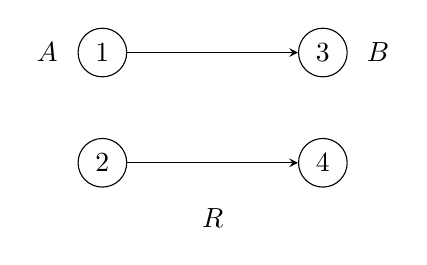
\begin{tikzpicture}[scale=0.7]
		\node[circle,draw] (a1) at (0,0) {1};
		\node[circle,draw] (a2) at (0,-2) {2};
		\node[circle,draw] (b1) at (4,0) {3};
		\node[circle,draw] (b2) at (4,-2) {4};

		\draw[->,>=stealth] (a1) -- (b1);
		\draw[->,>=stealth] (a2) -- (b2);

		\node at (-1,0) {$A$};
		\node at (5,0) {$B$};
		\node at (2,-3) {$R$};
	\end{tikzpicture}
\end{center}
\sol
The diagram shows a graphical representation of the relation $R$. The nodes on the left represent elements of set $A$, and the nodes on the right represent elements of set $B$. The directed edges (arrows) represent the ordered pairs in the relation $R$.

\subsection{Number of Possible Relations}

For finite sets $A$ and $B$, the number of possible binary relations from $A$ to $B$ is determined by the number of subsets of $A \times B$.

\nt{
	If $|A| = m$ and $|B| = n$, then $|A \times B| = m \cdot n$. The number of possible relations is the number of subsets of $A \times B$, which is $2^{|A \times B|} = 2^{m \cdot n}$.
}

\ex{Counting Relations}{
	If $A = \{1, 2\}$ and $B = \{x, y, z\}$, how many possible relations are there from $A$ to $B$?
}
\sol
$|A| = 2$ and $|B| = 3$, so $|A \times B| = 2 \times 3 = 6$.
The number of possible relations is $2^6 = 64$.

\subsection{Types of Relations}

\begin{itemize}
	\item \textbf{Reflexive Relation:} A relation $R$ on a set $A$ is reflexive if $(a, a) \in R$ for all $a \in A$.
	\item \textbf{Symmetric Relation:} A relation $R$ on a set $A$ is symmetric if $(a, b) \in R$ implies $(b, a) \in R$ for all $a, b \in A$.
	\item \textbf{Transitive Relation:} A relation $R$ on a set $A$ is transitive if $(a, b) \in R$ and $(b, c) \in R$ implies $(a, c) \in R$ for all $a, b, c \in A$.
	\item \textbf{Equivalence Relation} A relation that is reflexive, symmetric and transitive.
\end{itemize}

\section{Properties That Relations Can Satisfy}

\subsection{Reflexive Relations}

\dfn{Reflexive Relation}{
	A relation $R$ on a set $A$ is called \textbf{reflexive} if for all $x \in A$, $xRx$ (or $(x,x) \in R$). In other words, every element in the set is related to itself.
}

\ex{Example of Reflexive Relations}{
	Let $A = \{1, 2, 3\}$.
	\begin{itemize}
		\item $R_1 = \{(1,1), (2,2), (3,3)\}$ is reflexive.
		\item $R_2 = \{(1,1), (2,2), (3,3), (2,3)\}$ is also reflexive.
	\end{itemize}
}
\nt{
	The key characteristic of a reflexive relation is that every element of the set *must* be related to itself.  The presence of other relations (like (2,3) in $R_2$) doesn't affect the reflexivity.
}

\qs{How many possible reflexive relations are there for a set A if $|A| = n$?}{
}
\sol{
	\begin{itemize}
		\item  If $|A| = n$, then $|A \times A| = n^2$. This represents all possible ordered pairs in the Cartesian product of A with itself.
		\item All possible relations on A is $2^{n^2}$, since a relation is a subset of $A \times A$, and the number of subsets of a set with $n^2$ elements is $2^{n^2}$.
		\item If a relation $R$ on $A$ is reflexive, then for all $a_i \in A$, $(a_i, a_i)$ must be in $R$, where $1 \le i \le n$.
		\item We must consider the rest of the pairs, which are $n^2 - n$.
		\item Therefore, the number of reflexive relations is $2^{(n^2 - n)}$.  This is because the $n$ pairs of the form $(a_i, a_i)$ are *required* for reflexivity, leaving $n^2 - n$ other pairs that may or may not be present.
	\end{itemize}

}

\subsection{Symmetric Relations}

\dfn{Symmetric Relation}{
	A relation $R$ on a set $A$ is \textbf{symmetric} if for all $x, y \in A$, if $(x, y) \in R$, then $(y, x) \in R$. In simpler terms, if $x$ is related to $y$, then $y$ must also be related to $x$.
}

\ex{Examples of Symmetric Relations}{
	Let $A = \{1, 2, 3\}$.
	\begin{itemize}
		\item $R_1 = \{(1,2), (2,1), (3,1), (1,3)\}$ is symmetric, but not reflexive.
		\item $R_2 = \{(1,1), (2,2), (3,3)\}$ is reflexive and symmetric.
	\end{itemize}
}

\qs{How many symmetric relations are there?}{
}

\sol{
	\begin{itemize}
		\item For pairs of the form $(a_i, a_i)$, we can either include or exclude them. There are $n$ such pairs, leading to $2^n$ possibilities.
		\item For the remaining $n^2 - n$ elements, they must come in pairs: $(a_i, a_j)$ and $(a_j, a_i)$.
		\item There are $\frac{1}{2}(n^2 - n)$ such pairs.
		\item For each of these $\frac{1}{2}(n^2 - n)$ pairs, we can either include both $(a_i, a_j)$ and $(a_j, a_i)$ or exclude both.
		\item Thus, there are $2^{\frac{1}{2}(n^2 - n)}$ choices for these pairs.
		\item  The total number of symmetric relations is $2^n \cdot 2^{\frac{1}{2}(n^2 - n)} = 2^{n + \frac{1}{2}(n^2-n)} =  2^{\frac{1}{2}(n^2 + n)}$.
	\end{itemize}
}

\subsection{Antisymmetric Relations}

\dfn{Antisymmetric Relation}{
	A relation $R$ on a set $A$ is \textbf{antisymmetric} if for all $a, b \in A$, if $(a, b) \in R$ and $(b, a) \in R$, then $a = b$.  This means that the only way for both $(a,b)$ and $(b,a)$ to be in the relation is if $a$ and $b$ are the same element.
}

\ex{Examples of Antisymmetric Relations}{
	Let $A = \{1, 2, 3\}$.
	\begin{itemize}
		\item $R_1 = \{(1,2), (2,1), (1,1)\}$ is not symmetric and not antisymmetric.
		\item $R_2 = \{(1,2), (1,3)\}$ is antisymmetric.
		\item $R_3 = \{(1,1), (2,2)\}$ is symmetric and antisymmetric.
	\end{itemize}
}

\qs{How many antisymmetric relations are there?}{
}

\sol{
	\begin{itemize}
		\item For pairs $(a_i, a_i)$, it doesn't matter if we include them or not. There are $n$ such pairs, so $2^n$ possibilities.
		\item For pairs $(a_i, a_j)$ where $i \neq j$, if we include one pair, we cannot include the other.
		\item There are $\frac{1}{2}(n^2 - n)$ such pairs of pairs.
		\item For each pair of pairs, there are three options:
		      \begin{enumerate}
			      \item Place $(a_i, a_j) \in R$.
			      \item Place $(a_j, a_i) \in R$.
			      \item Place neither.
		      \end{enumerate}
		\item Thus, there are $3^{\frac{1}{2}(n^2-n)}$ options for these pairs.
		\item The total number of antisymmetric relations will be $2^n \cdot 3^{\frac{1}{2}(n^2 - n)}$.
	\end{itemize}
}

\nt{
	\begin{tabular}{c|c}
		Note              &     \\
		\hline
		T $\rightarrow$ T & : T \\
		T $\rightarrow$ F & : F \\
		F $\rightarrow$ T & : T \\
		F $\rightarrow$ F & : T
	\end{tabular}
}

\section{Relations and Divisibility}

\subsection{Defining a Relation}

\ex{Example: Divisors of 12}{
	Let $A = \{1, 2, 3, 4, 6, 12\}$. This set contains all the positive divisors of 12.
}

\dfn{Definition: Relation on A}{
	Define a relation $R$ on $A$ as $(x, y) \in R$ if and only if $x | y$, which means "$x$ exactly divides $y$".
}

\nt{
	The notation $(x, y) \in R$ is often written as $xRy$. The relation $R$ in this context represents the divisibility relation.
}

\subsection{Properties of the Relation}

\nt{
	We will check if the relation $R$ is reflexive, antisymmetric, and transitive.
}

\begin{itemize}
	\item \textbf{Reflexive:} For all $x \in A$, $x | x$, so $(x, x) \in R$. Thus, $R$ is reflexive.
	\item \textbf{Antisymmetric:} If $x | y$ and $y | x$, then $x = y$. So, if $(x, y) \in R$ and $(y, x) \in R$, then $x = y$. Thus, $R$ is antisymmetric.
	\item \textbf{Transitive:} If $x | y$ and $y | z$, then $x | z$. So, if $(x, y) \in R$ and $(y, z) \in R$, then $(x, z) \in R$. Thus, $R$ is transitive.
\end{itemize}

\ex{Examples of Pairs in R}{
	Some pairs in $R$ include $(2, 4)$, $(4, 12)$, and consequently, $(2, 12)$ due to transitivity.
}

\subsection{Counting Ordered Pairs}

\qs{Question: Number of Ordered Pairs}{
	How many ordered pairs occur in $R$?
}

\sol{
	We can use prime factorization to determine the number of ordered pairs. Given $12 = 2^2 \cdot 3^1$, if $(c, d) \in R$, then $c = 2^m 3^n$ and $d = 2^p 3^q$ where:
	\begin{itemize}
		\item $0 \leq m \leq p \leq 2$
		\item $0 \leq n \leq q \leq 1$
	\end{itemize}

	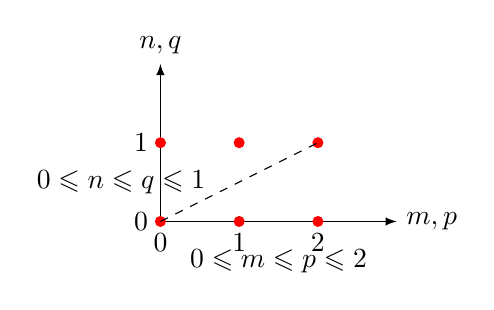
\begin{tikzpicture}
		\draw[->] (0,0) -- (3,0) node[right] {$m, p$};
		\draw[->] (0,0) -- (0,2) node[above] {$n, q$};

		\foreach \x in {0,1,2}
		\draw (\x cm,1pt) -- (\x cm,-1pt) node[anchor=north] {$\x$};
		\foreach \y in {0,1}
		\draw (1pt,\y cm) -- (-1pt,\y cm) node[anchor=east] {$\y$};

		\fill[red] (0,0) circle (2pt);
		\fill[red] (1,0) circle (2pt);
		\fill[red] (2,0) circle (2pt);
		\fill[red] (0,1) circle (2pt);
		\fill[red] (1,1) circle (2pt);
		\fill[red] (2,1) circle (2pt);

		\draw[dashed] (0,0) -- (2,1);

		\node at (1.5,-0.5) {$0 \leq m \leq p \leq 2$};
		\node at (-0.5,0.5) {$0 \leq n \leq q \leq 1$};

	\end{tikzpicture}

	For $m$ and $p$, we can pick from $\{0, 1, 2\}$. The number of ways to choose $m$ and $p$ such that $0 \leq m \leq p \leq 2$ is given by $\binom{3-1+2}{2} = \binom{4}{2} = 6$.
	For $n$ and $q$, we pick from $\{0, 1\}$. The number of ways to choose $n$ and $q$ such that $0 \leq n \leq q \leq 1$ is given by $\binom{2-1+2}{2} = \binom{3}{2} = 3$.
	Total number of ordered pairs = $6 \times 3 = 18$.
}

\subsection{Generalization for 1800}
\qs{Question: Generalization}{Consider the number $1800 = 2^3 \cdot 3^2 \cdot 5^2$. How many ordered pairs are there such that one divides the other?}
\sol{
	Let $1800 = 2^3 \cdot 3^2 \cdot 5^2$. If $(c,d) \in R$ such that $ c|d$ and both divide 1800, we have $c = 2^r 3^s 5^t$ and $d = 2^u 3^v 5^w$.
	Then
	\begin{itemize}
		\item $0 \leq r \leq u \leq 3$
		\item $0 \leq s \leq v \leq 2$
		\item $0 \leq t \leq w \leq 2$
	\end{itemize}
	The number of ways to choose $r$ and $u$ is $\binom{4-1+2}{2} = \binom{5}{2} = 10$.
	The number of ways to choose $s$ and $v$ is $\binom{3-1+2}{2} = \binom{4}{2} = 6$.
	The number of ways to choose $t$ and $w$ is $\binom{3-1+2}{2} = \binom{4}{2} = 6$.
	Thus, the total number of such ordered pairs is $10 \times 6 \times 6 = 360$.
}

\section{Function}

\nt{
	The notes were taken on Tuesday, 4 March 2025, at 11:08.
}

\subsection{Definition of a Function}

\dfn{Function}{
	For non-empty sets $A$ and $B$, a function (or mapping) $f$ from $A$ to $B$, denoted as $f: A \rightarrow B$, is a relation in which every element of $A$ appears exactly once as a component of an ordered pair in $R$ (where R is likely the set of ordered pairs defining the function).
}

\subsection{Example 1}

\ex{Example 1}{
	Let $A = \{1, 2, 3\}$ and $B = \{w, x, y, z\}$. Define a function $f$ as follows:
	\[
		f = \{(1, w), (2, x), (3, x)\}
	\]
}
\ex{Example 2}{
	Consider the relation $R$:
	\[
		R = \{(1, w), (2, w), (3, x), (3, z)\}
	\]
	This is \textit{not} a function because the element $3$ in set $A$ is mapped to two different elements ($x$ and $z$) in set $B$.
}

\subsection{Domain, Codomain, and Range}
Consider the function in the first Example.

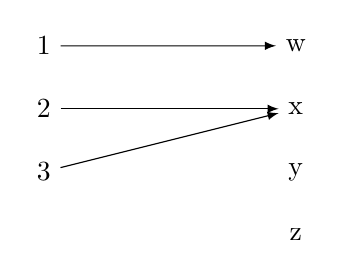
\begin{tikzpicture}[scale=0.8]

	\node (1) at (-0.5,1.5) {1};
	\node (2) at (-0.5,0.5) {2};
	\node (3) at (-0.5,-0.5) {3};

	\node (w) at (3.5,1.5) {w};
	\node (x) at (3.5,0.5) {x};
	\node (y) at (3.5,-0.5) {y};
	\node (z) at (3.5,-1.5) {z};

	\draw[->] (1) -- (w);
	\draw[->] (2) -- (x);
	\draw[->] (3) -- (x);
\end{tikzpicture}

\begin{itemize}
	\item $A$ is the \textbf{domain}.
	\item $B$ is the \textbf{codomain}.
	\item $f(A) = \{w, x\}$ is the \textbf{range} of $f$. The range is the set of all elements in $B$ that are mapped to by at least one element in $A$.  It is a subset of the codomain.
\end{itemize}

\subsection{Number of Possible Functions}

\qs{How Many Functions?}{
	How many functions are possible from set $A$ to set $B$?
}

\sol{
If $|A| = 3$ and $|B| = 4$, then the number of possible functions is $|B|^{|A|} = 4^3$. In General, if we have a set $A$ and $B$, the number of functions possible is $|B|^{|A|}$.

}

\subsection{One-to-One Functions (Injective Functions)}

\dfn{One-to-One Function (Injective)}{
	A function is one-to-one (injective) if each element of the codomain is mapped to by at most one element of the domain.  In other words, no two elements in the domain map to the same element in the codomain.
}

\begin{itemize}
	\item Example of an injective function:
\end{itemize}

\begin{tikzpicture}[scale=0.8]

	\node (1a) at (-0.5,1.5) {1};
	\node (2a) at (-0.5,0.5) {2};
	\node (3a) at (-0.5,-0.5) {3};

	\node (4b) at (3.5,1.5) {4};
	\node (5b) at (3.5,0.5) {5};
	\node (6b) at (3.5,-0.5) {6};

	\draw[->] (1a) -- (4b);
	\draw[->] (2a) -- (5b);
	\draw[->] (3a) -- (6b);
	\node[below= 0.1cm of 3a] {Injective};
\end{tikzpicture}
\begin{itemize}
	\item Example of a *non*-injective function:
\end{itemize}

\begin{tikzpicture}[scale=0.8]

	\node (1c) at (5.5,1.5) {1};
	\node (2c) at (5.5,0.5) {2};
	\node (3c) at (5.5,-0.5) {3};

	\node (4d) at (9.5,1.5) {4};
	\node (5d) at (9.5,0.5) {5};
	\node (6d) at (9.5,-0.5) {6};
	\node (7d) at (9.5,-1.5) {7};
	\draw[->] (1c) -- (4d);
	\draw[->] (2c) -- (5d);
	\draw[->] (3c) -- (5d);
	\node[below= 0.1cm of 3c] {Not injective};
\end{tikzpicture}

\subsection{Number of One-to-One Functions}
Consider Sets $A= \{1,2,3,4\}$ and $B = \{4,5,6,7,8\}$.
\qs{How many one to one functions?}{
	How many 1-to-1 functions are there from A to B?
}

\sol{
	$5 \cdot 4 \cdot 3 \cdot 2$. This can be expressed generally as:

	For the first element in A, there are 5 choices in B.
	For the second element in A, there are 4 remaining choices in B (since it must be one-to-one).
	For the third element in A, there are 3 remaining choices in B.
	For the fourth element in A, there are 2 remaining choices in B.
}

\subsection{General Case}

\nt{
	Let:
	\begin{itemize}
		\item $A = \{a_1, a_2, \dots, a_n\}$, where $n \leq m$
		\item $B = \{b_1, b_2, \dots, b_m\}$
	\end{itemize}
	Then, the number of one-to-one functions from $A$ to $B$ is given by $P(m, n)$, which represents permutations of $m$ items taken $n$ at a time. This is calculated as:
	\[
		P(m, n) = \frac{m!}{(m-n)!} = m \cdot (m-1) \cdot (m-2) \dots (m-n+1)
	\]
	If $n>m$, there will be 0 one-to-one functions, as the pigeon hole principle states.
}

\section{Surjective and Onto Functions}

\dfn{Surjective (Onto) Function}{
	A function \( f: A \rightarrow B \) is surjective (or onto) if for every element \( b \) in the codomain \( B \), there exists at least one element \( a \) in the domain \( A \) such that \( f(a) = b \). In other words, the range of \( f \) is equal to its codomain \( B \), or  \( f(A) = B \).
}

\ex{Example of Surjective and Non-Surjective Functions}{
	Consider the sets \( A = \{1, 2, 3, 4\} \) and \( B = \{x, y, z\} \).

	\begin{enumerate}
		\item Define \( f_1: A \rightarrow B \) as follows:
		      \( f_1(1) = x \), \( f_1(2) = y \), \( f_1(3) = z \), \( f_1(4) = z \)

		      This function IS surjective because every element in \( B \) has at least one corresponding element in \( A \).

		\item Define \( f_2: A \rightarrow B \) as follows:
		      \( f_2(1) = x \), \( f_2(2) = x \), \( f_2(3) = y \), \( f_2(4) = y \)

		      This function is NOT surjective (not onto) because the element \( z \in B \) has no pre-image in \( A \).
	\end{enumerate}
}

\qs{How to check for onto functions?}{
	How can we determine if a function is onto, especially when dealing with larger or infinite sets?
}
\sol{
One common method is using the Inclusion-Exclusion Principle. Another is to try and express an arbitrary element of the co-domain in terms of an element from the domain.

Consider sets \( A = \{a, b, c, d\} \) and \( B = \{1, 2, 3, 4\} \).  If we have a function \( f: A \rightarrow B \), then the total number of possible functions is \( |B|^{|A|} = 4^4 \).

To calculate the number of onto functions, we can use the Inclusion-Exclusion Principle.
}

\subsection{Inclusion-Exclusion Principle}

\nt{
	The Inclusion-Exclusion Principle is a counting technique which generalizes the familiar method of obtaining the number of elements in the union of two finite sets.
}
\ex{Inclusion-Exclusion Example (Number of Onto Functions)}{
For finite sets \( A \) and \( B \) where \( |A| = m \) and \( |B| = n \), and we want to find the number of onto functions \( f: A \rightarrow B \),  the formula derived from the Inclusion-Exclusion Principle is:

\[
	\sum_{k=0}^{n} (-1)^k \binom{n}{k} (n-k)^m
\]

Let's consider a simple example:
\(A = \{a,b,c\}\)
\(B = \{1,2,3\}\)
The number of functions is \( |B|^{|A|} = 3^3 = 27\)
\[
	\left( \binom{3}{0} 3^3 \right) - \left( \binom{3}{1} 2^3 \right) + \left( \binom{3}{2} 1^3 \right) - \left( \binom{3}{3} 0^3 \right)
\]
}

\section{Counting Problems}

\subsection{Elevator Problem}

\qs{Elevator Problem}{
	Seven people enter an elevator. The elevator will stop at four different floors. What is the probability that the elevator must stop at all four floors?
}

\sol{
	This problem is equivalent to finding the number of onto functions from a set of 7 people (objects) to a set of 4 floors (boxes).

	\begin{itemize}
		\item Let \( A \) represent the set of people, so \( |A| = 7 \).
		\item Let \( B \) represent the set of floors, so \( |B| = 4 \).
	\end{itemize}

	We want to find the number of onto functions from \( A \) to \( B \).  Using the Inclusion-Exclusion Principle:

	\[
		\sum_{k=0}^{4} (-1)^k \binom{4}{k} (4-k)^7
	\]
	The Total number of ways 7 people can get off on 4 floors is:
	\[
		4^7
	\]
	The probability that the elevator must stop on all floors is:
	\[
		\frac{\sum_{k=0}^{4} (-1)^k \binom{4}{k} (4-k)^7}{4^7}
	\]
}
\subsection{Dice Rolling Problem}

\qs{Dice Rolling Problem}{
	A die is tossed 12 times (or equivalently, 12 dice are tossed simultaneously). What is the probability of seeing all 6 faces?
}

\sol{
	This is analogous to finding the number of onto functions from a set of 12 tosses (objects) to a set of 6 faces (boxes).

	\begin{itemize}
		\item Let \( A \) represent the set of tosses, so \( |A| = 12 \).
		\item Let \( B \) represent the set of faces, so \( |B| = 6 \).
	\end{itemize}

	We want to find the number of onto functions from \( A \) to \( B \).  Using the Inclusion-Exclusion Principle:
	\[
		\sum_{k=0}^{6} (-1)^k \binom{6}{k} (6-k)^{12}
	\]
	The total number of possible outcomes when rolling a die 12 times is \( 6^{12} \).

	Therefore, the probability of seeing all 6 faces is:

	\[
		\frac{\sum_{k=0}^{6} (-1)^k \binom{6}{k} (6-k)^{12}}{6^{12}}
	\]
	This can also be expressed in terms of Stirling numbers of the second kind, denoted as \( S(n, k) \) or \( \begin{Bmatrix} n \\ k \end{Bmatrix} \), which counts the number of ways to partition a set of \( n \) objects into \( k \) non-empty subsets. The number of onto functions is \( 6! \cdot S(12, 6) \).
}
\dfn{Stirling Numbers of the Second Kind}{
	\( S(n, k) \) or \( \begin{Bmatrix} n \\ k \end{Bmatrix} \) represents the number of ways to partition a set of *n* objects into *k* non-empty subsets.
}
\nt{
	The formula to calculate Stirling numbers of the second kind is:

	\[ S(n, k) = \frac{1}{k!} \sum_{j=0}^{k} (-1)^{k-j} \binom{k}{j} j^n \]
}

\section{Where does this come from?}

\nt{
	If $A = \{a,b,c,d\}$ \\
	$B = \{1, 2, 3\}$ \\
	$\exists$ 36 onto functions
}

\qs{Question}{
	But if Boxes in B are identical? \\
	Then there are $\frac{36}{3!}$ to put 4 distinct objects in 3 identical containers.
}
\sol{

}

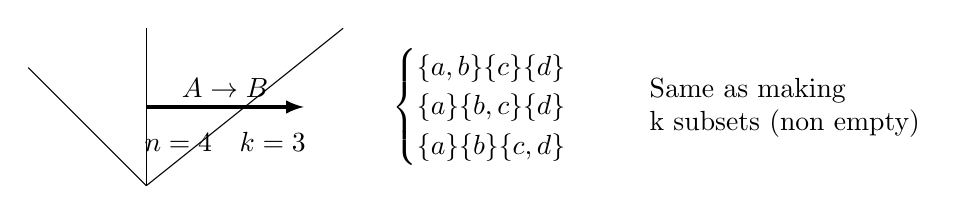
\begin{tikzpicture}
	\draw[->, very thick] (0,0) -- (2,0);
	\node[above] at (1,0) {$A \rightarrow B$};
	\node[below] at (1,-0.2) {$n=4 \quad k=3$};
	\draw (3,0) node[right] {
		$\begin{cases}
				\{a,b\} \{c\} \{d\} \\
				\{a\} \{b,c\} \{d\} \\
				\{a\} \{b\} \{c,d\}
			\end{cases}$
		\quad
		\begin{tabular}{l}
			Same as making \\
			k subsets (non empty)
		\end{tabular}
	};

	\draw (0,-1) -- (2.5,1);
	\draw (0,-1) -- (0,1);
	\draw (0,-1) -- (-1.5,0.5);
\end{tikzpicture}

\nt{
	\# of ways to partition $n$ distinct objects in $k$ parts.
}
\section{Stirling Number of the Second Kind}

\dfn{Stirling Number of the Second Kind}{
	\[
		S(n,k) = \frac{1}{k!} \sum_{j=0}^{k} (-1)^j \binom{k}{j} (k-j)^n
	\]
}

\nt{
	The Stirling number of the second kind, \( S(n,k) \), represents the number of ways to partition \( n \) distinct objects into \( k \) identical boxes.
}

\nt{
	Basic Properties:
	\begin{itemize}
		\item \( S(n,1) = S(n,n) = 1 \)
		\item Recursive Relation: \( S(n,k) = S(n-1, k-1) + k \cdot S(n-1, k) \) for \( 2 \leq k \leq n-1 \)
	\end{itemize}
}

\ex{Example}{
	For 6 objects and 3 identical containers:
	\[
		S(6,3) = S(5,2) + 3 \cdot S(5,3)
	\]
}

\nt{
	Understanding the Recursive Relation:
	\begin{itemize}
		\item One object is inserted alone, illustrating that configurations are the same.
		\item Once 3 people are placed, boxes become distinct, allowing 3 places to insert the last person.
	\end{itemize}
}

\chapter{Discrete Calculus}

\qs{Sums for Discrete Functions?}{
	Can we define concepts analogous to derivatives for discrete functions?
}

\sol
\begin{itemize}
	\item $\Delta f(x) = f(x+1) - f(x) \implies$ \boxed{\text{FORWARD DIFFERENCE}}
	\item $\Delta^2 f(x) = \Delta[\Delta f(x)] = \Delta[f(x+1) - f(x)] = [f(x+2) - f(x+1)] - [f(x+1) - f(x)]$
	      \begin{align*}
		       & = f(x+2) - 2f(x+1) + f(x)
	      \end{align*}
\end{itemize}

\dfn{Shift Operator}{
Define operator $E$ such that:
\[ E[f(x)] = f(x+1) \]
And in general
\[E^n[f(x)] = f(x+n)\]
h so $\Delta f(x) = E[f(x)] - f(x) = (E-I)f(x)$
}

\begin{itemize}
	\item $\Delta^n [f(x)] = (E-I)^n f(x)$
	      \begin{align*}
		       & = \left[ E^n[f(x)] - \binom{n}{1}E^{n-1}[f(x)] + ... + (-1)^k\binom{n}{k}E^{n-k}f(x) \right]
	      \end{align*}
\end{itemize}

\ex{Example}{
$\Delta^2(x^3) = (E-I)^2(x^3)=[E^2 - 2EI + I^2]x^3$

$=E^2x^3 -2(x+1)^3 + x^3 = 6x+6$
}

\nt{
	\begin{itemize}
		\item The forward difference of \(x^3\) results in \(6x + 6\).
		\item Compare this with the second derivative \(\frac{d^2}{dx^2}x^3 = 6x\).
	\end{itemize}
}

\section{Analogies to Continuous Calculus}

\subsection{The Difference Operator}

\dfn{Difference Operator}{
	The difference operator, denoted by $\Delta$, is the discrete analog of the derivative.  For a function $f(x)$, it is defined as:
	\[
		\Delta[f(x)] = f(x+1) - f(x)
	\]
	More generally, for a step size $h$, we have $\Delta_h[f(x)] = f(x+h) - f(x)$.  Here, we are primarily concerned with the case $h=1$.
}

\nt{
	The difference operator gives the change in the function's value when the input increases by 1.  It's a "forward difference."
}

\ex{Example: Linear Function}{
	Consider $f(x) = 6x + 6$. Then,
	\[
		\Delta[f(x)] = f(x+1) - f(x) = (6(x+1) + 6) - (6x + 6) = 6x + 6 + 6 - 6x - 6 = 6
	\]
}

\ex{Example: Quadratic Function}{
	Consider $f(x)=x^2$
	\[
		\Delta[f(x)] = f(x+1)-f(x) = (x+1)^2 -x^2 = x^2 + 2x +1 - x^2 = 2x+1
	\]
}

\subsection{Product Rule Analogy}

In continuous calculus, the product rule states:
\[
	\frac{d}{dx}[f(x)g(x)] = f'(x)g(x) + f(x)g'(x)
\]

We seek a discrete analog.  Let's try:

\[
	\Delta[f(x)g(x)] = f(x+1)g(x+1) - f(x)g(x)
\]

We can manipulate this expression by adding and subtracting a "clever zero": $f(x)g(x+1) - f(x)g(x+1)$.

\begin{align*}
	\Delta[f(x)g(x)] & = f(x+1)g(x+1) - f(x)g(x+1) + f(x)g(x+1) - f(x)g(x) \\
	                 & = g(x+1)[f(x+1) - f(x)] + f(x)[g(x+1) - g(x)]       \\
	                 & = g(x+1)\Delta[f(x)] + f(x)\Delta[g(x)]
\end{align*}

\thm{Discrete Product Rule}{
	\[
		\Delta[f(x)g(x)] = g(x+1)\Delta[f(x)] + f(x)\Delta[g(x)]
	\]
}
\nt{
	Notice the slight difference from the continuous product rule.  One of the terms uses $g(x+1)$ instead of $g(x)$.
}

\subsection{The Discrete Analog of $e^x$}

In continuous calculus, the function $e^{kx}$ has the property that $\frac{d}{dx}e^{kx} = ke^{kx}$.  That is, it's an eigenfunction of the derivative operator. We seek a discrete analog.

Consider $f(x) = a^x$, where $a \in \mathbb{Z}^+$. Then
\[
	\Delta[f(x)] = a^{x+1} - a^x = a^x(a - 1)
\]

If we choose $a=2$, we have
\[
	\Delta[2^x] = 2^x(2-1) = 2^x
\]
Thus, $2^x$ is the discrete analog of $e^x$, as it is an eigenfunction of the difference operator with eigenvalue 1. We can say "2 is the discrete $e$".

\subsection{Falling Factorials}

\dfn{Falling Factorial}{
	The falling factorial, denoted by $x^{(n)}$, is defined as:
	\[
		x^{(n)} = x(x-1)(x-2)\cdots(x-n+1)
	\]
	where $n$ is a non-negative integer. It's a product of $n$ terms. If n=0, $x^{(0)} = 1$
}

\ex{Example}{
	$x^{(3)} = x(x-1)(x-2)$
}

\dfn{When is the Falling Factorial Zero?}{
	If $n > c$, one of the terms in the product will be zero, specifically when $c-k = 0$ for some $k$. This results in:

	\begin{equation}
		c^{(n)} = 0, \quad \text{for } n > c.
	\end{equation}

	Thus, for any constant $c$, if $n > c$, we have $c^{(n)} = 0$.
}

Now, let's compute the difference of a falling factorial:

\begin{align*}
	\Delta[x^{(n)}] & = (x+1)^{(n)} - x^{(n)}                                 \\
	                & = (x+1)(x)(x-1)\cdots(x-n+2) - x(x-1)(x-2)\cdots(x-n+1) \\
	                & = x(x-1)\cdots(x-n+2)[(x+1) - (x-n+1)]                  \\
	                & = x(x-1)\cdots(x-n+2)[n]                                \\
	                & = n x^{(n-1)}
\end{align*}

\thm{Difference of Falling Factorial}{
	\[
		\Delta[x^{(n)}] = nx^{(n-1)}
	\]
}
This is analogous to the power rule in continuous calculus: $\frac{d}{dx}x^n = nx^{n-1}$.

\subsection{Standard Basis vs. Falling Factorial Basis}

Polynomials can be expressed in different bases.

\begin{itemize}
	\item \textbf{Standard Basis:}  $\{1, x, x^2, x^3, \dots\}$
	\item \textbf{Falling Factorial Basis:} $\{1, x^{(1)}, x^{(2)}, x^{(3)}, \dots\}$
\end{itemize}

\qs{Converting Between Bases}{
	How do we convert a polynomial from the standard basis to the falling factorial basis, and vice-versa?
}
\sol{
Let's consider a cubic polynomial as an example. Suppose we have a polynomial in the standard basis:

\[ P(x) = Ax^3 + Bx^2 + Cx + D \]

We want to express it in the falling factorial basis:

\[ P(x) = A'x^{(3)} + B'x^{(2)} + C'x^{(1)} + D' \]

We can do this by successively applying the difference operator and evaluating at $x=0$.

\begin{enumerate}
	\item $P(0) = D = D'$
	\item $\Delta[P(x)] = 3Ax^2 + 2Bx + C = 3A'x^{(2)} + 2B'x^{(1)} + C'$.  Evaluating at $x=0$, we get $\Delta[P(0)] = C = C'$.
	\item $\Delta^2[P(x)] = 6Ax + 2B = 6A'x^{(1)} + 2B'$. Evaluating at $x=0$, we get $\Delta^2[P(0)] = 2B = 2B'$, so $B = B'$.
	\item $\Delta^3[P(x)] = 6A = 6A'$.  Thus, $A=A'$.
\end{enumerate}

Alternatively, we can express the falling factorials in terms of the standard basis:

\begin{itemize}
	\item $x^{(1)} = x$
	\item $x^{(2)} = x(x-1) = x^2 - x$
	\item $x^{(3)} = x(x-1)(x-2) = x^3 - 3x^2 + 2x$
\end{itemize}
Then, we can solve for $x$, $x^2$, and $x^3$ in terms of the falling factorials and substitute.

}

\ex{Example: Conversion}{
	Convert $P(x) = 3x^3 - x^2 + 6x + 5$ to the falling factorial basis.

	\sol
	First expand the falling factorial terms:
	$x^{(1)} = x$
	$x^{(2)} = x(x-1) = x^2 - x$
	$x^{(3)} = x(x-1)(x-2) = x^3-3x^2+2x$

	We can setup a system of equations, or we can use the method of successive differences.
	Method 1: System of Equations
	We want to find $A, B, C, D$ such that
	$3x^3-x^2+6x+5 = A x^{(3)} + B x^{(2)} + Cx^{(1)} + D$
	Substituting the expanded forms:
	$3x^3 - x^2 + 6x + 5 = A(x^3 - 3x^2 + 2x) + B(x^2 - x) + Cx + D$
	$3x^3 - x^2 + 6x + 5 = Ax^3 + (-3A+B)x^2 + (2A-B+C)x + D$
	Comparing coefficients:
	\begin{itemize}
		\item $A=3$
		\item $-3A+B=-1 \Rightarrow -9+B=-1 \Rightarrow B=8$
		\item $2A-B+C=6 \Rightarrow 6-8+C=6 \Rightarrow C=8$
		\item $D=5$
	\end{itemize}
	So, $3x^3 - x^2 + 6x + 5 = 3x^{(3)} + 8x^{(2)} + 8x^{(1)} + 5$.

	Method 2: Successive Differences
	\begin{enumerate}
		\item $P(x) = 3x^3 - x^2 + 6x + 5$, $P(0) = 5$, so $D=5$.
		\item $\Delta P(x) = 3(x+1)^3 - (x+1)^2 + 6(x+1) + 5 - (3x^3-x^2+6x+5) = 9x^2+5x+8$, and $\Delta P(0) = 8$, so $C=8$.
		\item $\Delta^2 P(x) = 9(x+1)^2+5(x+1)+8 - (9x^2+5x+8) = 18x + 14$, $\Delta^2 P(0) = 14$, and we know $\Delta^2 x^{(2)} = 2$, so $14/2= B = 7$ is incorrect (from the previous derivation it should be 8, so the method from the original document is not perfectly correct).
		\item $\Delta^3 P(x) = 18(x+1)+14-(18x+14)=18$, $\Delta^3 x^{(3)} = 6$. Thus $18/6=A=3$, as $A=3$
	\end{enumerate}
	The second method is incorrect, so we should rely on the first one.

}

\subsection{Matrix Representation of Basis Change}
We can represent the change of basis using a matrix.  Consider converting a cubic polynomial from the falling factorial basis to the standard basis.

\[
	\begin{pmatrix}
		1 \\ x \\ x^2 \\ x^3
	\end{pmatrix}
	=
	\begin{pmatrix}
		1 & 0  & 0  & 0 \\
		0 & 1  & 0  & 0 \\
		0 & -1 & 1  & 0 \\
		0 & 2  & -3 & 1
	\end{pmatrix}
	\begin{pmatrix}
		1 \\ x^{(1)} \\ x^{(2)} \\ x^{(3)}
	\end{pmatrix}
\]

The matrix entries are the coefficients when expressing $x^n$ in terms of the falling factorials. The inverse of this matrix would perform the conversion from the standard basis to the falling factorial basis.
Since $\Delta x^{(n)} = nx^{(n-1)}$, we have:
\[
	\Delta \begin{pmatrix} x^{(0)} \\ x^{(1)} \\ x^{(2)} \\ x^{(3)} \end{pmatrix} = \begin{pmatrix} 0 \\ 1 \\ 2x^{(1)} \\ 3x^{(2)} \end{pmatrix} = \begin{pmatrix} 0 & 0 & 0 & 0 \\ 1 & 0 & 0 & 0 \\ 0 & 2 & 0 & 0 \\ 0 & 0 & 3 & 0\end{pmatrix} \begin{pmatrix}  x^{(0)} \\ x^{(1)} \\ x^{(2)} \\ x^{(3)}\end{pmatrix}
\]
\subsection{General Basis}

Consider a general basis of the form: $\{1, (x-x_0), (x-x_0)(x-x_1), (x-x_0)(x-x_1)(x-x_2), \dots \}$

\ex{Example}{
	Consider the basis $\{1, x, x(x-2), x(x-2)(x-3) \}$. We can expand $x^2$ in this basis. We look for coefficients $A, B, C$ such that:

	$x^2 = A \cdot 1 + B \cdot x + C \cdot x(x-2)$
	$x^2= A + Bx +Cx^2-2Cx$
	$x^2 = Cx^2 + (B-2C)x +A $

	Comparing coefficients,
	$C=1$
	$B-2C=0 \rightarrow B-2=0 \rightarrow B=2$
	$A=0$

	$x^2 = 2x + x(x-2)$

	Consider the expansion of $x^2$ in terms of falling factorial:

	$x^2 = x + x(x-1) = x^{(1)} + x^{(2)}$
}

\section{Linear Combinations}

\subsection{Generating Sets}

\dfn{Generating Set}{
	A generating set of a vector space $V$ is a set of vectors such that every vector in $V$ can be written as a linear combination of the vectors in the generating set.
}

\nt{
	The provided notes explore a specific summation and its connection to integration. The core idea is to demonstrate how a discrete sum can approximate a definite integral. Let's break it down step by step.
}
\ex{Summation Formula}{
Given a summation:
\[
	\sum_{x=a}^{b} x^{(n)} = \frac{x^{(n+1)}}{n+1} \Big|_a^{b+1}
\]
where $x^{(n)}$ likely represents the falling factorial power, defined as $x^{(n)} = x(x-1)(x-2)...(x-n+1)$.
}

\thm{Falling Factorial Power Summation}{
For a falling factorial power $x^{(n)} = x(x-1)...(x-n+1)$, the summation from $x=a$ to $b$ is given by:
\[
	\sum_{x=a}^{b} x^{(n)} = \frac{x^{(n+1)}}{n+1} \Big|_{a}^{b+1} = \frac{(b+1)^{(n+1)}}{n+1} - \frac{a^{(n+1)}}{n+1}
\]
}

\nt{ The right-hand side of the initial equation resembles the evaluation of a definite integral. This suggests a connection between the discrete summation and continuous integration.}

\ex{Specific Example}{
The notes also present a more concrete example:

\[
	\sum_{1}^{n} x = \sum_1^n \frac{\Delta x^{(2)}}{2} = \frac{1}{2} x^{(2)} \Big|_1^{n+1}
\]

Here, $\Delta x^{(2)}$ likely represents the difference $ (x+1)^{(2)}-x^{(2)} $.
}

\thm{Sum of First n Natural Numbers}{
The sum of the first 'n' natural numbers can be represented and calculated using the falling factorial as follows:
\[
	\sum_{x=1}^{n} x = \frac{1}{2} x(x-1+1) \Big|_{1}^{n+1}= \frac{1}{2}[(n+1)(n) - (1)(0)] = \frac{n(n+1)}{2}
\]

}

\nt{
	This establishes the familiar formula for the sum of the first 'n' natural numbers. The connection to the falling factorial and the structure resembling integration (evaluation at upper and lower bounds) is highlighted.
}

\subsection{Connection to Integration}
\nt{
The general form $\sum_{x=a}^{b} x^{(n)} = \frac{x^{(n+1)}}{n+1} \Big|_a^{b+1}$ strongly mirrors the power rule of integration: $\int x^n dx = \frac{x^{n+1}}{n+1} + C$. The discrete sum of falling factorials is analogous to the definite integral. The limits of summation ($a$ and $b$) correspond to the limits of integration. The $+1$ on the upper bound in the summation formula mimics the nature of discrete steps versus continuous evaluation.
}

\ex{Illustrative Example - Sum of First n Integers}{

	Consider the summation of the first 'n' integers:
	\[
		\sum_{x=1}^{n} x
	\]
	This can be viewed as an approximation of the integral:
	\[
		\int_{1}^{n} x \, dx
	\]

}
\begin{tikzpicture}
	\begin{axis}[
			axis lines = left,
			xlabel = $x$,
			ylabel = {$f(x) = x$},
			xmin=0, xmax=6,
			ymin=0, ymax=6,
			xtick={1,2,3,4,5},
			ytick={1,2,3,4,5},
			width=8cm, height=8cm,
			clip=false
		]
		\addplot [
			domain=0:5,
			samples=100,
			color=blue,
		]
		{x};
		\addplot[
			ycomb,
			color=red,
			mark=*,
		]
		coordinates {
				(1,1)
				(2,2)
				(3,3)
				(4,4)
				(5,5)
			};

		\draw[dashed] (axis cs:1,0) -- (axis cs:1,1);
		\draw[dashed] (axis cs:2,0) -- (axis cs:2,2);
		\draw[dashed] (axis cs:3,0) -- (axis cs:3,3);
		\draw[dashed] (axis cs:4,0) -- (axis cs:4,4);
		\draw[dashed] (axis cs:5,0) -- (axis cs:5,5);

		\node[right] at (axis cs: 5,5) {$f(x) = x$};
		\node[above] at (axis cs: 1,1) {$\bullet$};
		\node[above] at (axis cs: 2,2) {$\bullet$};
		\node[above] at (axis cs: 3,3) {$\bullet$};
		\node[above] at (axis cs: 4,4) {$\bullet$};
		\node[above] at (axis cs: 5,5) {$\bullet$};
		\node[below] at (axis cs:1, 0) {1};
		\node[below] at (axis cs:2, 0) {2};
		\node[below] at (axis cs:3, 0) {3};
		\node[below] at (axis cs:4, 0) {4};
		\node[below] at (axis cs:5, 0) {5};

		\addplot[
			only marks,
			mark=*,
			color = black
		] coordinates{(1,0) (2,0) (3,0) (4,0) (5,0)};
	\end{axis}
\end{tikzpicture}

\nt{
	The blue line represents the continuous function $f(x) = x$.  The red dots represent the discrete values at integer points. The summation $\sum_{x=1}^{n} x$ adds up the y-values of these red dots. The integral $\int_{1}^{n} x \, dx$ calculates the area under the blue line from $x=1$ to $x=n$.  As 'n' increases, and the discrete steps become smaller, the summation becomes a better approximation of the integral.
}

\qs{Relationship between Summation and Integration}{
	How does the discrete summation relate to the definite integral?
}

\sol
The discrete summation can be seen as a Riemann sum approximation of the definite integral.  Specifically, it's akin to a right Riemann sum where the width of each rectangle is 1. The falling factorial summation formula provides a closed-form expression for this particular type of Riemann sum.


\nt{
	In essence, the notes demonstrate a fundamental concept in calculus: the connection between discrete sums and continuous integrals.  The falling factorial provides a bridge between these two worlds, allowing for a discrete analogue of the power rule of integration.
}

\section{Second Order Homogeneous Recurrence Relation with Constant Coefficients}

\subsection{General Form}

A second-order homogeneous recurrence relation with constant coefficients is an equation of the form:
$$a_n + a_{n-1} - 6a_{n-2} = 0$$

\subsection{Solving the Recurrence Relation}

To solve this, we assume a solution of the form $a_n = Cr^n$, where $C$ and $r$ are constants. Substituting this into the recurrence relation, we get:
$$Cr^n + Cr^{n-1} - 6Cr^{n-2} = 0$$
Dividing by $Cr^{n-2}$ (assuming $C \neq 0$ and $r \neq 0$), we obtain the characteristic equation:
$$r^2 + r - 6 = 0$$
Factoring the quadratic, we have:
$$(r+3)(r-2) = 0$$
Thus, the roots are $r_1 = 2$ and $r_2 = -3$.

\subsection{General Solution}

The general solution is a linear combination of the solutions corresponding to each root:
$$a_n = C_1(2)^n + C_2(-3)^n$$
where $C_1$ and $C_2$ are constants determined by initial conditions.

\subsection{Specific Solution with Initial Conditions}

Suppose we are given the initial conditions $a_0 = -1$ and $a_1 = 8$. We can use these to find $C_1$ and $C_2$:
\begin{align*}
	a_0 = C_1(2)^0 + C_2(-3)^0 & = C_1 + C_2 = -1  \\
	a_1 = C_1(2)^1 + C_2(-3)^1 & = 2C_1 - 3C_2 = 8
\end{align*}
Solving this system of equations:
From the first equation, $C_1 = -1 - C_2$. Substituting this into the second equation:
$$2(-1 - C_2) - 3C_2 = 8$$
$$-2 - 2C_2 - 3C_2 = 8$$
$$-5C_2 = 10$$
$$C_2 = -2$$
Then, $C_1 = -1 - (-2) = 1$.
Therefore, the specific solution is:
$$a_n = (1)(2)^n + (-2)(-3)^n = 2^n - 2(-3)^n$$

\section{Recurrence Relation Example 1}

\subsection{Problem Statement}

Consider the recurrence relation $a_{n+2} = a_{n+1} + a_n$ for $n \geq 0$, with initial conditions $a_0 = 0$ and $a_1 = 1$.

\subsection{Solving the Recurrence Relation}

Assume a solution of the form $a_n = Cr^n$. Substituting into the recurrence relation, we get:
$$Cr^{n+2} = Cr^{n+1} + Cr^n$$
Dividing by $Cr^n$, we obtain the characteristic equation:
$$r^2 = r + 1$$
$$r^2 - r - 1 = 0$$
Using the quadratic formula, we find the roots:
$$r = \frac{-(-1) \pm \sqrt{(-1)^2 - 4(1)(-1)}}{2(1)} = \frac{1 \pm \sqrt{5}}{2}$$
Thus, the roots are $r_1 = \frac{1 + \sqrt{5}}{2}$ and $r_2 = \frac{1 - \sqrt{5}}{2}$.

\subsection{General Solution}

The general solution is:
$$a_n = C_1\left(\frac{1 + \sqrt{5}}{2}\right)^n + C_2\left(\frac{1 - \sqrt{5}}{2}\right)^n$$

\subsection{Specific Solution with Initial Conditions}

We have $a_0 = 0$ and $a_1 = 1$.
\begin{align*}
	a_0 = C_1\left(\frac{1 + \sqrt{5}}{2}\right)^0 + C_2\left(\frac{1 - \sqrt{5}}{2}\right)^0 & = C_1 + C_2 = 0                                                                       \\
	a_1 = C_1\left(\frac{1 + \sqrt{5}}{2}\right)^1 + C_2\left(\frac{1 - \sqrt{5}}{2}\right)^1 & = C_1\left(\frac{1 + \sqrt{5}}{2}\right) + C_2\left(\frac{1 - \sqrt{5}}{2}\right) = 1
\end{align*}
From the first equation, $C_2 = -C_1$. Substituting this into the second equation:
$$C_1\left(\frac{1 + \sqrt{5}}{2}\right) - C_1\left(\frac{1 - \sqrt{5}}{2}\right) = 1$$
$$C_1\left(\frac{1 + \sqrt{5} - (1 - \sqrt{5})}{2}\right) = 1$$
$$C_1\left(\frac{2\sqrt{5}}{2}\right) = 1$$
$$C_1\sqrt{5} = 1$$
$$C_1 = \frac{1}{\sqrt{5}}$$
Then, $C_2 = -\frac{1}{\sqrt{5}}$.
Therefore, the specific solution is:
$$a_n = \frac{1}{\sqrt{5}}\left(\frac{1 + \sqrt{5}}{2}\right)^n - \frac{1}{\sqrt{5}}\left(\frac{1 - \sqrt{5}}{2}\right)^n = \frac{1}{\sqrt{5}}\left[\left(\frac{1 + \sqrt{5}}{2}\right)^n - \left(\frac{1 - \sqrt{5}}{2}\right)^n\right]$$
This is the closed-form expression for the Fibonacci sequence.

\chapter{Recurrence Relations}

\section{Recurrence Relation with Complex Roots}

\subsection{Problem Statement}

Consider the recurrence relation $a_n = 2a_{n-1} - 2a_{n-2}$ for $n \geq 2$, with initial conditions $a_0 = 1$ and $a_1 = 2$.

\subsection{Solving the Recurrence Relation}

Assume a solution of the form $a_n = Cr^n$. Substituting into the recurrence relation, we get:
$$Cr^n = 2Cr^{n-1} - 2Cr^{n-2}$$
Dividing by $Cr^{n-2}$, we obtain the characteristic equation:
$$r^2 - 2r + 2 = 0$$
Using the quadratic formula, we find the roots:
$$r = \frac{-(-2) \pm \sqrt{(-2)^2 - 4(1)(2)}}{2(1)} = \frac{2 \pm \sqrt{4 - 8}}{2} = \frac{2 \pm \sqrt{-4}}{2} = \frac{2 \pm 2i}{2} = 1 \pm i$$
Thus, the roots are $r_1 = 1 + i$ and $r_2 = 1 - i$.

\subsection{General Solution}

Since the roots are complex, we can express them in polar form. Let $r = x + iy$. Then, $|r| = \sqrt{x^2 + y^2}$ and $\theta = \arctan(\frac{y}{x})$.
In our case, $r_1 = 1 + i$, so $|r_1| = \sqrt{1^2 + 1^2} = \sqrt{2}$ and $\theta_1 = \arctan(\frac{1}{1}) = \frac{\pi}{4}$.
Thus, $r_1 = \sqrt{2}(\cos(\frac{\pi}{4}) + i\sin(\frac{\pi}{4}))$ and $r_2 = \sqrt{2}(\cos(\frac{\pi}{4}) - i\sin(\frac{\pi}{4}))$.
The general solution is:
$$a_n = C_1[\sqrt{2}(\cos(\frac{\pi}{4}) + i\sin(\frac{\pi}{4}))]^n + C_2[\sqrt{2}(\cos(\frac{\pi}{4}) - i\sin(\frac{\pi}{4}))]^n$$
Using De Moivre's Theorem, we have:
$$a_n = C_1 (\sqrt{2})^n (\cos(\frac{n\pi}{4}) + i\sin(\frac{n\pi}{4})) + C_2 (\sqrt{2})^n (\cos(\frac{n\pi}{4}) - i\sin(\frac{n\pi}{4}))$$
$$a_n = (\sqrt{2})^n [(C_1 + C_2)\cos(\frac{n\pi}{4}) + i(C_1 - C_2)\sin(\frac{n\pi}{4})]$$
Let $K_1 = C_1 + C_2$ and $K_2 = i(C_1 - C_2)$. Then,
$$a_n = (\sqrt{2})^n [K_1\cos(\frac{n\pi}{4}) + K_2\sin(\frac{n\pi}{4})]$$

\subsection{Specific Solution with Initial Conditions}

We have $a_0 = 1$ and $a_1 = 2$.
\begin{align*}
	a_0 = (\sqrt{2})^0 [K_1\cos(\frac{0\pi}{4}) + K_2\sin(\frac{0\pi}{4})] & = K_1\cos(0) + K_2\sin(0) = K_1 = 1                              \\
	a_1 = (\sqrt{2})^1 [K_1\cos(\frac{1\pi}{4}) + K_2\sin(\frac{1\pi}{4})] & = \sqrt{2} [K_1\cos(\frac{\pi}{4}) + K_2\sin(\frac{\pi}{4})] = 2
\end{align*}
Since $K_1 = 1$, we have:
$$\sqrt{2} [\cos(\frac{\pi}{4}) + K_2\sin(\frac{\pi}{4})] = 2$$
$$\sqrt{2} [\frac{\sqrt{2}}{2} + K_2\frac{\sqrt{2}}{2}] = 2$$
$$1 + K_2 = 2$$
$$K_2 = 1$$
Therefore, the specific solution is:
$$a_n = (\sqrt{2})^n [\cos(\frac{n\pi}{4}) + \sin(\frac{n\pi}{4})]$$

\section{Recurrence Relation with Repeated Roots}

\subsection{Problem Statement}

Consider the recurrence relation $a_{n+2} = 4a_{n+1} - 4a_n$ with initial conditions $a_0 = 1$ and $a_1 = 3$.

\subsection{Solving the Recurrence Relation}

Assume a solution of the form $a_n = Cr^n$. Substituting into the recurrence relation, we get:
$$Cr^{n+2} = 4Cr^{n+1} - 4Cr^n$$
Dividing by $Cr^n$, we obtain the characteristic equation:
$$r^2 - 4r + 4 = 0$$
$$(r-2)^2 = 0$$
Thus, we have a repeated root $r = 2$ with multiplicity $k = 2$.

\subsection{General Solution}

When there is a repeated root, the general solution is of the form:
$$a_n = C_1(2)^n + C_2n(2)^n$$

\subsection{Specific Solution with Initial Conditions}

We have $a_0 = 1$ and $a_1 = 3$.
\begin{align*}
	a_0 = C_1(2)^0 + C_2(0)(2)^0 & = C_1 = 1         \\
	a_1 = C_1(2)^1 + C_2(1)(2)^1 & = 2C_1 + 2C_2 = 3
\end{align*}
Since $C_1 = 1$, we have:
$$2(1) + 2C_2 = 3$$
$$2C_2 = 1$$
$$C_2 = \frac{1}{2}$$
Therefore, the specific solution is:
$$a_n = (2)^n + \frac{1}{2}n(2)^n$$

\subsection{Linear Independence of Solutions}
\qs{Question}{How do we show that $2^n$ and $n2^n$ are linearly independent eigenfunctions?}
\sol
We can use the Wronskian determinant to show that $2^n$ and $n2^n$ are linearly independent.  The Wronskian is calculated as follows:
$$W(n) = \begin{vmatrix}
		2^n     & n2^n         \\
		2^{n+1} & (n+1)2^{n+1}
	\end{vmatrix} = 2^n(n+1)2^{n+1} - n2^n2^{n+1} = (n+1)2^{2n+1} - n2^{2n+1} = 2^{2n+1}$$
Since $W(n) \neq 0$ for all $n$, the functions $2^n$ and $n2^n$ are linearly independent.

\section{Inhomogeneous Recurrence Relations}

\subsection{Problem Statement}

Consider the inhomogeneous recurrence relation $a_n + a_{n-1} = 3n^2$ for $n \geq 1$, with initial condition $a_0 = 7$.

\subsection{Solving the Recurrence Relation}

We can find a particular solution by summing the recurrence relation:
\begin{align*}
	a_1 & = a_0 + f(1)                            \\
	a_2 & = a_1 + f(2) = a_0 + f(1) + f(2)        \\
	a_3 & = a_2 + f(3) = a_0 + f(1) + f(2) + f(3) \\
	    & \vdots                                  \\
	a_n & = a_0 + \sum_{k=1}^{n} f(k)
\end{align*}
In our case, $a_0 = 7$ and $f(n) = 3n^2$. Thus,
$$a_n = 7 + \sum_{k=1}^{n} 3k^2 = 7 + 3\sum_{k=1}^{n} k^2$$
We know that $\sum_{k=1}^{n} k^2 = \frac{n(n+1)(2n+1)}{6}$. Therefore,
$$a_n = 7 + 3\left[\frac{n(n+1)(2n+1)}{6}\right] = 7 + \frac{n(n+1)(2n+1)}{2}$$
$$a_n = 7 + \frac{2n^3 + 3n^2 + n}{2}$$


\section*{Recurrence Relations}

\subsection*{Solving Inhomogeneous Recurrences}

\dfn{Linear Inhomogeneous Recurrence Relation}{
A linear inhomogeneous recurrence relation with constant coefficients is of the form:
\[ c_k a_n + c_{k-1} a_{n-1} + \dots + c_0 a_{n-k} = f(n) \]
where $c_i$ are constants, $c_k \neq 0$, $c_0 \neq 0$, and $f(n)$ is a non-zero function of $n$.
The associated homogeneous recurrence relation is:
\[ c_k a_n + c_{k-1} a_{n-1} + \dots + c_0 a_{n-k} = 0 \]
}

\thm{General Solution of Inhomogeneous Recurrence}{
The general solution $a_n$ to an inhomogeneous recurrence relation is the sum of the general solution to the associated homogeneous recurrence relation, $a_n^{(h)}$, and a particular solution to the inhomogeneous recurrence relation, $a_n^{(p)}$.
\[ a_n = a_n^{(h)} + a_n^{(p)} \]
The constants in $a_n^{(h)}$ are determined using the initial conditions after finding the complete general solution $a_n$.
}

\ex{Recurrence Relation $a_n - a_{n-1} = 3n^2$ (Iteration Method)}{
We are asked to solve the recurrence relation $a_n - a_{n-1} = 3n^2$ for $n \ge 1$, with the initial condition $a_0 = 7$.

\sol
This is a first-order linear inhomogeneous recurrence relation. We can solve it by iteration (also known as telescoping sum).
Let $f(n) = 3n^2$. The relation is $a_n = a_{n-1} + f(n)$.
We can write out the first few terms:
\begin{align*} a_1 &= a_0 + f(1) = 7 + 3(1^2) \\ a_2 &= a_1 + f(2) = (a_0 + f(1)) + f(2) = 7 + 3(1^2) + 3(2^2) \\ a_3 &= a_2 + f(3) = (a_0 + f(1) + f(2)) + f(3) = 7 + 3(1^2) + 3(2^2) + 3(3^2) \end{align*}
In general, we can see the pattern:
\[ a_n = a_0 + \sum_{i=1}^n f(i) = 7 + \sum_{i=1}^n 3i^2 = 7 + 3 \sum_{i=1}^n i^2 \]
We use the formula for the sum of the first $n$ squares: $\sum_{i=1}^n i^2 = \frac{n(n+1)(2n+1)}{6}$.
Substituting this into our expression for $a_n$:
\[ a_n = 7 + 3 \left( \frac{n(n+1)(2n+1)}{6} \right) \]
\[ a_n = 7 + \frac{n(n+1)(2n+1)}{2} \]
We can expand this expression:
\[ a_n = 7 + \frac{n(2n^2 + 3n + 1)}{2} = 7 + \frac{2n^3 + 3n^2 + n}{2} \]
\[ a_n = \frac{14 + 2n^3 + 3n^2 + n}{2} = n^3 + \frac{3}{2}n^2 + \frac{1}{2}n + 7 \]
The solution to the recurrence relation is $a_n = 7 + \frac{n(n+1)(2n+1)}{2}$.
}

\ex{Recurrence Relation $a_n - 3a_{n-1} = 5(7)^n$ (Method of Undetermined Coefficients)}{
Solve the recurrence relation $a_n - 3a_{n-1} = 5(7)^n$ for $n \ge 1$, with $a_0 = 2$.

\sol
This is a first-order linear inhomogeneous recurrence relation. We use the method of undetermined coefficients.

\begin{enumerate}
    \item \textbf{Find the homogeneous solution $a_n^{(h)}$:}
    The associated homogeneous equation is $a_n^{(h)} - 3a_{n-1}^{(h)} = 0$.
    The characteristic equation is $r - 3 = 0$, which gives the root $r=3$.
    The general homogeneous solution is $a_n^{(h)} = C(3)^n$, where C is a constant.

    \item \textbf{Find a particular solution $a_n^{(p)}$:}
    The inhomogeneous term is $f(n) = 5(7)^n$. Since $f(n)$ is of the form $(\text{constant}) \times 7^n$, and $7$ is not a root of the characteristic equation ($r=3$), we guess a particular solution of the form $a_n^{(p)} = \alpha (7)^n$.
    Substitute $a_n^{(p)}$ into the original recurrence relation:
    \[ \alpha (7)^n - 3 [\alpha (7)^{n-1}] = 5(7)^n \]
    Divide by $7^{n-1}$ (assuming $n \ge 1$):
    \[ \alpha (7) - 3 \alpha = 5(7) \]
    \[ 7\alpha - 3\alpha = 35 \]
    \[ 4\alpha = 35 \]
    \[ \alpha = \frac{35}{4} \]
    So, the particular solution is $a_n^{(p)} = \frac{35}{4} (7)^n$.

    \item \textbf{Find the general solution $a_n$:}
    The general solution is $a_n = a_n^{(h)} + a_n^{(p)} = C(3)^n + \frac{35}{4} (7)^n$.

    \item \textbf{Use the initial condition to find C:}
    We are given $a_0 = 2$. Substitute $n=0$ into the general solution:
    \[ a_0 = C(3)^0 + \frac{35}{4} (7)^0 \]
    \[ 2 = C(1) + \frac{35}{4} (1) \]
    \[ 2 = C + \frac{35}{4} \]
    \[ C = 2 - \frac{35}{4} = \frac{8}{4} - \frac{35}{4} = -\frac{27}{4} \]

    \item \textbf{Write the final solution:}
    Substituting the value of C back into the general solution:
    \[ a_n = -\frac{27}{4} (3)^n + \frac{35}{4} (7)^n \]
\end{enumerate}
}

\ex{Recurrence Relation $a_n - 3a_{n-1} = 5(3)^n$ (Resonant Case)}{
Solve the recurrence relation $a_n - 3a_{n-1} = 5(3)^n$ for $n \ge 1$, with $a_0 = 2$.

\sol
This is similar to the previous example, but the inhomogeneous term involves the root of the characteristic equation.

\begin{enumerate}
    \item \textbf{Find the homogeneous solution $a_n^{(h)}$:}
    The associated homogeneous equation is $a_n^{(h)} - 3a_{n-1}^{(h)} = 0$.
    The characteristic equation is $r - 3 = 0$, giving the root $r=3$.
    The general homogeneous solution is $a_n^{(h)} = C(3)^n$.

    \item \textbf{Find a particular solution $a_n^{(p)}$:}
    The inhomogeneous term is $f(n) = 5(3)^n$. Since the base $3$ matches the characteristic root $r=3$ (with multiplicity $m=1$), we must modify our guess for the particular solution. Instead of $\alpha(3)^n$, we guess $a_n^{(p)} = \alpha n^m (3)^n = \alpha n (3)^n$.
    Substitute $a_n^{(p)}$ into the original recurrence relation:
    \[ \alpha n (3)^n - 3 [\alpha (n-1) (3)^{n-1}] = 5(3)^n \]
    Divide by $3^{n-1}$:
    \[ \alpha n (3) - 3 [\alpha (n-1)] = 5(3) \]
    \[ 3\alpha n - 3\alpha (n-1) = 15 \]
    \[ 3\alpha n - 3\alpha n + 3\alpha = 15 \]
    \[ 3\alpha = 15 \]
    \[ \alpha = 5 \]
    So, the particular solution is $a_n^{(p)} = 5n (3)^n$.

    \nt{If we had tried $a_n^{(p)} = \beta(3)^n$, substituting would give $\beta(3)^n - 3\beta(3)^{n-1} = \beta(3)^n - \beta(3)^n = 0$. Setting this equal to $5(3)^n$ gives $0 = 5(3)^n$, which is impossible. This confirms the need for the modification factor $n$.}

    \item \textbf{Find the general solution $a_n$:}
    The general solution is $a_n = a_n^{(h)} + a_n^{(p)} = C(3)^n + 5n(3)^n = (C+5n)3^n$.

    \item \textbf{Use the initial condition to find C:}
    We are given $a_0 = 2$. Substitute $n=0$:
    \[ a_0 = (C+5(0))3^0 \]
    \[ 2 = (C)(1) \]
    \[ C = 2 \]

    \item \textbf{Write the final solution:}
    Substituting $C=2$ back into the general solution:
    \[ a_n = (2+5n)3^n \]
\end{enumerate}
}

\subsection*{Summation via Recurrence Relations}

We can sometimes evaluate summations by framing them as recurrence relations.

\ex{Finding a Closed Form for $\sum_{i=1}^n i^2$}{
Find a closed-form expression for the sum $S_n = \sum_{i=1}^n i^2$.

\sol
Let $a_n = \sum_{i=1}^n i^2$. We define $a_0 = 0$.
For $n \ge 1$, we have the relationship:
\[ a_n = \sum_{i=1}^n i^2 = \left( \sum_{i=1}^{n-1} i^2 \right) + n^2 = a_{n-1} + n^2 \]
This gives us the recurrence relation $a_n - a_{n-1} = n^2$ with $a_0 = 0$. This is a linear inhomogeneous recurrence relation.

\begin{enumerate}
    \item \textbf{Homogeneous solution $a_n^{(h)}$:}
    The homogeneous equation is $a_n^{(h)} - a_{n-1}^{(h)} = 0$.
    The characteristic equation is $r-1=0$, so $r=1$.
    The homogeneous solution is $a_n^{(h)} = C(1)^n = C$.

    \item \textbf{Particular solution $a_n^{(p)}$:}
    The inhomogeneous term is $f(n) = n^2$, a polynomial of degree 2.
    Since the characteristic root is $r=1$ (multiplicity $m=1$), we guess a particular solution of the form $a_n^{(p)} = n^m (\text{polynomial of degree 2}) = n(Bn^2 + Dn + E)$. Let's use the constants as in the notes: $a_n^{(p)} = n(Dn^2 + Cn + B) = Dn^3 + Cn^2 + Bn$. (Note: the constants B,C,D here correspond to D,C,B in the notes' guess $Bn+Cn^2+Dn^3$. Let's stick to $Dn^3 + Cn^2 + Bn$ to match the standard form).
    Substitute into $a_n - a_{n-1} = n^2$:
    \[ (Dn^3 + Cn^2 + Bn) - [D(n-1)^3 + C(n-1)^2 + B(n-1)] = n^2 \]
    Expand $(n-1)^3 = n^3 - 3n^2 + 3n - 1$ and $(n-1)^2 = n^2 - 2n + 1$.
    \[ D(n^3 - (n^3 - 3n^2 + 3n - 1)) + C(n^2 - (n^2 - 2n + 1)) + B(n - (n-1)) = n^2 \]
    \[ D(3n^2 - 3n + 1) + C(2n - 1) + B(1) = n^2 \]
    \[ (3D)n^2 + (-3D + 2C)n + (D - C + B) = 1 \cdot n^2 + 0 \cdot n + 0 \]
    Equating coefficients:
    \begin{itemize}
        \item Coefficient of $n^2$: $3D = 1 \implies D = 1/3$.
        \item Coefficient of $n$: $-3D + 2C = 0 \implies -3(1/3) + 2C = 0 \implies -1 + 2C = 0 \implies C = 1/2$.
        \item Constant term: $D - C + B = 0 \implies 1/3 - 1/2 + B = 0 \implies -1/6 + B = 0 \implies B = 1/6$.
    \end{itemize}
    The particular solution is $a_n^{(p)} = \frac{1}{3}n^3 + \frac{1}{2}n^2 + \frac{1}{6}n$.

    \item \textbf{General solution $a_n$:}
    $a_n = a_n^{(h)} + a_n^{(p)} = A + \frac{1}{3}n^3 + \frac{1}{2}n^2 + \frac{1}{6}n$. (Using A for the homogeneous constant).

    \item \textbf{Use initial condition $a_0 = 0$:}
    $a_0 = A + 0 + 0 + 0 = 0 \implies A = 0$.

    \item \textbf{Final solution:}
    $a_n = \frac{1}{3}n^3 + \frac{1}{2}n^2 + \frac{1}{6}n$.
    We can factor this expression:
    \[ a_n = \frac{2n^3 + 3n^2 + n}{6} = \frac{n(2n^2 + 3n + 1)}{6} = \frac{n(n+1)(2n+1)}{6} \]
\end{enumerate}
This confirms the well-known formula for the sum of the first $n$ squares.
}

\section*{Generating Functions}

\dfn{Ordinary Generating Function (OGF)}{
The ordinary generating function (OGF) for an infinite sequence $a_0, a_1, a_2, \dots$ is the formal power series:
\[ G(x) = \sum_{n=0}^\infty a_n x^n = a_0 + a_1 x + a_2 x^2 + \dots \]
}

\dfn{Exponential Generating Function (EGF)}{
The exponential generating function (EGF) for an infinite sequence $a_0, a_1, a_2, \dots$ is the formal power series:
\[ \hat{G}(x) = \sum_{n=0}^\infty a_n \frac{x^n}{n!} = a_0 + a_1 \frac{x}{1!} + a_2 \frac{x^2}{2!} + \dots \]
EGFs are particularly useful for problems involving arrangements or distributions of distinct objects.
}

\subsection*{Basic Generating Functions and Operations}

Some fundamental generating functions:
\begin{itemize}
    \item Sequence $1, 1, 1, \dots$ (i.e., $a_n = 1$ for all $n \ge 0$):
    OGF: $\sum_{n=0}^\infty 1 \cdot x^n = 1 + x + x^2 + \dots = \frac{1}{1-x}$.
    \item Sequence $1, c, c^2, c^3, \dots$ (i.e., $a_n = c^n$):
    OGF: $\sum_{n=0}^\infty c^n x^n = \sum_{n=0}^\infty (cx)^n = \frac{1}{1-cx}$.
    \item Finite Sequence $1, 1, \dots, 1$ (n+1 ones), $0, 0, \dots$:
    OGF: $1 + x + x^2 + \dots + x^n = \frac{1-x^{n+1}}{1-x}$.
    \item Sequence $0, 1, 2, 3, \dots$ (i.e., $a_n = n$):
    We can obtain this by differentiating the OGF for $1, 1, 1, \dots$ and multiplying by $x$.
    $\frac{d}{dx} \left( \frac{1}{1-x} \right) = \frac{1}{(1-x)^2} = 1 + 2x + 3x^2 + \dots = \sum_{n=0}^\infty (n+1)x^n$. (This is the OGF for $1, 2, 3, \dots$)
    Multiplying by $x$ shifts the sequence and introduces a leading zero:
    $x \cdot \frac{1}{(1-x)^2} = x + 2x^2 + 3x^3 + \dots = \sum_{n=1}^\infty n x^n$. This is the OGF for $0, 1, 2, 3, \dots$.
    \item Sequence $0, 1, 4, 9, \dots$ (i.e., $a_n = n^2$):
    Apply the operation $x \frac{d}{dx}$ to the OGF for $a_n=n$:
    $G_{n^2}(x) = x \frac{d}{dx} \left( \frac{x}{(1-x)^2} \right)$
    Using the quotient rule: $\frac{d}{dx} \left( \frac{x}{(1-x)^2} \right) = \frac{1 \cdot (1-x)^2 - x \cdot 2(1-x)(-1)}{(1-x)^4} = \frac{(1-x)^2 + 2x(1-x)}{(1-x)^4} = \frac{(1-x)(1-x+2x)}{(1-x)^4} = \frac{1+x}{(1-x)^3}$.
    So, $G_{n^2}(x) = x \cdot \frac{1+x}{(1-x)^3} = \frac{x(1+x)}{(1-x)^3}$.
    This is the OGF for $0^2, 1^2, 2^2, 3^2, \dots$.
\end{itemize}

\nt{
Operations on Generating Functions:
\begin{itemize}
    \item Addition: $A(x)+B(x) = \sum (a_n+b_n)x^n$. Corresponds to adding sequences term-wise.
    \item Multiplication by $x^k$: $x^k A(x) = \sum a_n x^{n+k} = \sum a_{n-k} x^n$. Shifts sequence $a_n$ right by $k$ positions, filling with zeros.
    \item Differentiation: $A'(x) = \sum n a_n x^{n-1}$.
    \item Integration: $\int A(x) dx = \sum \frac{a_n}{n+1} x^{n+1} + C$.
    \item Convolution: $A(x)B(x) = (\sum a_n x^n)(\sum b_n x^n) = \sum c_n x^n$, where $c_n = \sum_{k=0}^n a_k b_{n-k}$.
\end{itemize}
The operation $x \frac{d}{dx}$ applied to $A(x) = \sum a_n x^n$ yields $x A'(x) = \sum n a_n x^n$. The resulting generating function corresponds to the sequence $0, a_1, 2a_2, 3a_3, \dots$.
}

\subsection*{Applications to Combinatorial Problems}

\ex{Donut Selection (Ordinary Generating Functions)}{
How many ways are there to select 26 donuts from 4 types (say A, B, C, D) such that we select an even number of type C donuts and at least 6 type D donuts?

\sol
This is a selection problem where the order does not matter and items of the same type are indistinguishable. We use Ordinary Generating Functions. Let $x$ represent a donut. We want to find the coefficient of $x^{26}$ in the product of the generating functions for each type, representing the constraints.

\begin{itemize}
    \item Type A: No restrictions. We can choose $0, 1, 2, \dots$ donuts.
    GF: $A(x) = 1 + x + x^2 + x^3 + \dots = \frac{1}{1-x}$.
    \item Type B: No restrictions.
    GF: $B(x) = 1 + x + x^2 + x^3 + \dots = \frac{1}{1-x}$.
    \item Type C: Even number must be chosen ($0, 2, 4, \dots$).
    GF: $C(x) = 1 + x^2 + x^4 + x^6 + \dots = \sum_{k=0}^\infty (x^2)^k = \frac{1}{1-x^2}$.
    \item Type D: At least 6 must be chosen ($6, 7, 8, \dots$).
    GF: $D(x) = x^6 + x^7 + x^8 + \dots = x^6(1 + x + x^2 + \dots) = \frac{x^6}{1-x}$.
\end{itemize}

The overall generating function $G(x)$ is the product of these individual GFs:
\[ G(x) = A(x) B(x) C(x) D(x) = \left(\frac{1}{1-x}\right) \left(\frac{1}{1-x}\right) \left(\frac{1}{1-x^2}\right) \left(\frac{x^6}{1-x}\right) \]
\[ G(x) = \frac{x^6}{(1-x)^3 (1-x^2)} \]
We can simplify the denominator: $1-x^2 = (1-x)(1+x)$.
\[ G(x) = \frac{x^6}{(1-x)^3 (1-x)(1+x)} = \frac{x^6}{(1-x)^4 (1+x)} \]
We need the coefficient of $x^{26}$ in $G(x)$. This is equivalent to finding the coefficient of $x^{20}$ in the expansion of $H(x) = \frac{1}{(1-x)^4 (1+x)}$.
We use partial fraction decomposition for $H(x)$:
\[ \frac{1}{(1-x)^4 (1+x)} = \frac{A}{1+x} + \frac{B}{1-x} + \frac{C}{(1-x)^2} + \frac{D}{(1-x)^3} + \frac{E}{(1-x)^4} \]
Multiplying by $(1-x)^4 (1+x)$ gives:
\[ 1 = A(1-x)^4 + B(1+x)(1-x)^3 + C(1+x)(1-x)^2 + D(1+x)(1-x) + E(1+x) \]
We can find the constants by substituting values for $x$ or comparing coefficients.
\begin{itemize}
    \item Set $x=1$: $1 = E(1+1) = 2E \implies E = 1/2$.
    \item Set $x=-1$: $1 = A(1-(-1))^4 = A(2^4) = 16A \implies A = 1/16$.
    \item Using values found in the thought process (derived by solving a system of equations): $B = 1/16$, $C = 1/8$, $D = 1/4$.
\end{itemize}
So, $H(x) = \frac{1/16}{1+x} + \frac{1/16}{1-x} + \frac{1/8}{(1-x)^2} + \frac{1/4}{(1-x)^3} + \frac{1/2}{(1-x)^4}$.

Now we find the coefficient of $x^{20}$, denoted by $[x^{20}]$, in each term using the generalized binomial theorem $(1-z)^{-k} = \sum_{n=0}^\infty \binom{n+k-1}{n} z^n = \sum_{n=0}^\infty \binom{n+k-1}{k-1} z^n$ and $(1+x)^{-1} = \sum_{n=0}^\infty (-1)^n x^n$.
\begin{itemize}
    \item $[x^{20}] \frac{1/16}{1+x} = \frac{1}{16} (-1)^{20} = \frac{1}{16}$.
    \item $[x^{20}] \frac{1/16}{1-x} = \frac{1}{16} (1) = \frac{1}{16}$.
    \item $[x^{20}] \frac{1/8}{(1-x)^2} = \frac{1}{8} \binom{20+2-1}{20} = \frac{1}{8} \binom{21}{20} = \frac{1}{8} (21) = \frac{21}{8} = \frac{42}{16}$.
    \item $[x^{20}] \frac{1/4}{(1-x)^3} = \frac{1}{4} \binom{20+3-1}{20} = \frac{1}{4} \binom{22}{20} = \frac{1}{4} \binom{22}{2} = \frac{1}{4} \frac{22 \times 21}{2} = \frac{231}{4} = \frac{924}{16}$.
    \item $[x^{20}] \frac{1/2}{(1-x)^4} = \frac{1}{2} \binom{20+4-1}{20} = \frac{1}{2} \binom{23}{20} = \frac{1}{2} \binom{23}{3} = \frac{1}{2} \frac{23 \times 22 \times 21}{3 \times 2 \times 1} = \frac{1}{2} (23 \times 11 \times 7) = \frac{1771}{2} = \frac{14168}{16}$.
\end{itemize}
The total coefficient $[x^{20}] H(x)$ is the sum:
\[ \frac{1}{16} + \frac{1}{16} + \frac{42}{16} + \frac{924}{16} + \frac{14168}{16} = \frac{1+1+42+924+14168}{16} = \frac{15136}{16} \]
\[ \frac{15136}{16} = 946 \]
Therefore, there are 946 ways to select the 26 donuts according to the given constraints.
}

\ex{Item Distribution (Exponential Generating Functions)}{
How many ways are there to distribute 12 distinct items into 3 labeled boxes (A, B, C) such that box A has at least 4 items, box B has at least 2 items, and box C has between 2 and 5 items (inclusive)?

\sol
Since the items are distinct and the boxes are labeled, this problem calls for Exponential Generating Functions (EGFs). Let the number of items in boxes A, B, C be $a, b, c$ respectively. We require $a+b+c=12$, with $a \ge 4$, $b \ge 2$, and $2 \le c \le 5$.

The EGF for each box represents the constraints on the number of items it can receive:
\begin{itemize}
    \item Box A (at least 4 items): $A(x) = \frac{x^4}{4!} + \frac{x^5}{5!} + \frac{x^6}{6!} + \dots = e^x - \left(1 + \frac{x}{1!} + \frac{x^2}{2!} + \frac{x^3}{3!}\right)$.
    \item Box B (at least 2 items): $B(x) = \frac{x^2}{2!} + \frac{x^3}{3!} + \frac{x^4}{4!} + \dots = e^x - \left(1 + \frac{x}{1!}\right)$.
    \item Box C (between 2 and 5 items): $C(x) = \frac{x^2}{2!} + \frac{x^3}{3!} + \frac{x^4}{4!} + \frac{x^5}{5!}$.
\end{itemize}

The overall EGF for the distribution is the product $G(x) = A(x) B(x) C(x)$. We are looking for the coefficient of $\frac{x^{12}}{12!}$ in $G(x)$. This coefficient is equal to the number of ways to distribute the 12 items. The coefficient of $x^{12}$ in $G(x)$ is $[x^{12}]G(x)$, and the number of ways is $12! \times [x^{12}]G(x)$.

While we could try to multiply these series or use their $e^x$ expressions, it's often simpler for fixed totals to use a combinatorial approach based on the definition of the EGF coefficient. The number of ways is the sum of multinomial coefficients over all valid compositions $(a, b, c)$ of 12:
Number of ways $= \sum_{\substack{a+b+c=12 \\ a\ge 4, b\ge 2 \\ 2 \le c \le 5}} \binom{12}{a, b, c}$, where $\binom{12}{a, b, c} = \frac{12!}{a! b! c!}$.

We list the possible values for $c$ and the corresponding constraints on $a$ and $b$:
\begin{itemize}
    \item If $c=2$: $a+b=10$, $a\ge 4, b\ge 2$. Possible $(a,b)$: $(8,2), (7,3), (6,4), (5,5), (4,6)$.
    \item If $c=3$: $a+b=9$, $a\ge 4, b\ge 2$. Possible $(a,b)$: $(7,2), (6,3), (5,4), (4,5)$.
    \item If $c=4$: $a+b=8$, $a\ge 4, b\ge 2$. Possible $(a,b)$: $(6,2), (5,3), (4,4)$.
    \item If $c=5$: $a+b=7$, $a\ge 4, b\ge 2$. Possible $(a,b)$: $(5,2), (4,3)$.
\end{itemize}

Now we calculate the multinomial coefficient for each case and sum them up:
\begin{itemize}
    \item Case c=2:
    $\binom{12}{8,2,2} = \frac{12!}{8!2!2!} = \frac{12 \cdot 11 \cdot 10 \cdot 9}{4} = 2970$
    $\binom{12}{7,3,2} = \frac{12!}{7!3!2!} = \frac{12 \cdot 11 \cdot 10 \cdot 9 \cdot 8}{12} = 7920$
    $\binom{12}{6,4,2} = \frac{12!}{6!4!2!} = \frac{12 \cdot 11 \cdot 10 \cdot 9 \cdot 8 \cdot 7}{48} = 13860$
    $\binom{12}{5,5,2} = \frac{12!}{5!5!2!} = \frac{12 \cdot 11 \cdot 10 \cdot 9 \cdot 8 \cdot 7 \cdot 6}{2 \cdot 120} = 16632$
    $\binom{12}{4,6,2} = \frac{12!}{4!6!2!} = 13860$
    Sum for c=2: $2970 + 7920 + 13860 + 16632 + 13860 = 55242$.

    \item Case c=3:
    $\binom{12}{7,2,3} = \frac{12!}{7!2!3!} = \frac{12 \cdot 11 \cdot 10 \cdot 9 \cdot 8}{12} = 7920$
    $\binom{12}{6,3,3} = \frac{12!}{6!3!3!} = \frac{12 \cdot 11 \cdot 10 \cdot 9 \cdot 8 \cdot 7}{36} = 18480$
    $\binom{12}{5,4,3} = \frac{12!}{5!4!3!} = \frac{12 \cdot 11 \cdot 10 \cdot 9 \cdot 8 \cdot 7 \cdot 6}{144} = 27720$
    $\binom{12}{4,5,3} = \frac{12!}{4!5!3!} = 27720$
    Sum for c=3: $7920 + 18480 + 27720 + 27720 = 81840$.

    \item Case c=4:
    $\binom{12}{6,2,4} = \frac{12!}{6!2!4!} = \frac{12 \cdot 11 \cdot 10 \cdot 9 \cdot 8 \cdot 7}{48} = 13860$
    $\binom{12}{5,3,4} = \frac{12!}{5!3!4!} = 27720$
    $\binom{12}{4,4,4} = \frac{12!}{4!4!4!} = \frac{12 \cdot 11 \cdot 10 \cdot 9 \cdot 8 \cdot 7 \cdot 6 \cdot 5}{576} = 34650$
    Sum for c=4: $13860 + 27720 + 34650 = 76230$.

    \item Case c=5:
    $\binom{12}{5,2,5} = \frac{12!}{5!2!5!} = 16632$
    $\binom{12}{4,3,5} = \frac{12!}{4!3!5!} = 27720$
    Sum for c=5: $16632 + 27720 = 44352$.
\end{itemize}

The total number of ways is the sum of the ways for each possible value of c:
Total ways = $55242 + 81840 + 76230 + 44352 = 257664$.

There are 257,664 ways to distribute the 12 distinct items according to the constraints.
}

\end{document}